% arara: pdflatex
% !arara: biber
% !arara: pdflatex
% How to run:
% 1) pdflatex "filename".tex
% 2) biber "filename"
% 3) pdflatex "filename".tex
% 4) pdflatex "filename".tex


\documentclass[x11names,twoside,english]{uiofysmaster}

\usepackage{tikz}
\usepackage{environ}
\usepackage{physics}
\usepackage{amssymb}
\usepackage{ulem}
\usepackage{cleveref}
\usepackage{mathtools}
% \usepackage{subfigure}
% \usepackage{enumitem}
\usepackage{todonotes}
\usepackage{siunitx}


\usepackage{graphicx}
\usepackage{caption}
\usepackage{subcaption}
\usepackage{pifont}
\usepackage[utf8]{inputenc}
\usepackage{wrapfig}
% \usepackage{natbib}
% \usepackage{usebib}
\usepackage{amsmath}
\usepackage{algorithmicx}
\usepackage{algorithm}
\usepackage[noend]{algpseudocode}
\usepackage{tabularx}





%%%%%%%%%%%%%%%%%%%%%%%%%%%%%%%%%%%%%%%%%%%%%%%%%%%%%%%%%%%%%%%%%%%%%%%%%%%%%%
%	New Commands
%%%%%%%%%%%%%%%%%%%%%%%%%%%%%%%%%%%%%%%%%%%%%%%%%%%%%%%%%%%%%%%%%%%%%%%%%%%%%%
\newcommand*\circled[1]{\tikz[baseline=(C.base)]\node[draw,circle,inner sep=1.2pt,line width=0.2mm,](C) {\small #1};\!}

% \newcommand\norm[1]{\left\lVert#1\right\rVert}


%%%%%%%%%%%%%%%%%%%%%%%%%%%%%%%%%%%%%%%%%%%%%%%%%%%%%%%%%%%%%%%%%%%
%Tikz settings
% =================================================
% Set up a few colours
\colorlet{lcfree}{Green3}
\colorlet{lcnorm}{Blue3}
\colorlet{lccong}{Red3}
% -------------------------------------------------
% Set up a new layer for the debugging marks, and make sure it is on
% top
\pgfdeclarelayer{marx}
% \pgfsetlayers{main,marx}
% A macro for marking coordinates (specific to the coordinate naming
% scheme used here). Swap the following 2 definitions to deactivate
% marks.
\providecommand{\cmark}[2][]{%
  \begin{pgfonlayer}{marx}
    \node [nmark] at (c#2#1) {#2};
  \end{pgfonlayer}{marx}
  }
\providecommand{\cmark}[2][]{\relax}


% TikZ environment initialisation
\usetikzlibrary{calc,fadings,decorations.pathreplacing,decorations.markings}
\usetikzlibrary{shapes,arrows,chains}
% \usetikzlibrary{fadings,shapes.arrows,shadows}
% \usetikzlibrary{arrows,external,pgfplots.groupplots,positioning}
% \usetikzlibrary{intersections}
\usetikzlibrary{decorations.pathmorphing,patterns}
% Setting colours used
\definecolor{royalBlue}{RGB}{65,105,225}
\definecolor{cadred}{RGB}{227,0,34}
\definecolor{slateGray}{RGB}{119,136,153}

% TikZ style def.
\tikzset{
    %Define style for boxes
    >=stealth,
    punkt/.style={
           rectangle,
           rounded corners,
           draw=white, very thick,
           text width=10em,
           minimum height=2em,
           text centered},
    % Define arrow style
    pil/.style={
           ->,
           >=stealth,
           thick,
           shorten <=2pt,
           shorten >=2pt},
    % Define a box style for grid
    box/.style={
          rectangle,
          draw=black,
          thin,
          minimum size=0.1cm},
    circ node/.style={
          circle,
          draw,
          inner sep=4pt},
    % style to apply some styles to each segment of a path
    spring1/.style={
      decoration={
        aspect=1,
        segment length=1.448cm,
        % segment length=0.38cm,
        amplitude=0.3cm,
        coil,
      },
    },
    spring2/.style={
      decoration={
        aspect=0.399,
        segment length=0.601cm,
        amplitude=0.75cm,
        coil,
      },
    },
    % style to add an arrow in the middle of a path
    mid arrow/.style={postaction={decorate,decoration={
          markings,
          mark=at position .3 with {\arrow[#1]{stealth}}
    }}},
    extended line/.style={shorten >=-#1,shorten <=-#1},
}
% TikZ environment initialisation END
%%%%%%%%%%%%%%%%%%%%%%%%%%%%%%%%%%%%%%%%%%%%%%%%%%%%%%%%%%%%%%%%%%
% %% references
\usepackage[style=authoryear,
            bibstyle=authoryear,
            backend=biber,
            % refsection=chapter,
            maxbibnames=99,
            maxnames=2,
            firstinits=true,
            uniquename=init,
            natbib=true,
            dashed=false]{biblatex}

%Fix citetitle style
\DeclareFieldFormat*{citetitle}{#1}

% \addbibresource{bibs/bibliography.bib}
% \addbibresource{bibs/extra.bib}
\addbibresource{bibs/bibliography.bib}
%%%%%%%%%%%%%%%%%%%%%%%%%%%%%%%%%%%%%%%%%%%%%%%%%%%%%%%%%%%%%%%%%%


\author{Gullik Vetvik Killie}
\title{A Parallel Multigrid Poisson Solver for PINC, a Particle-in-Cell Model}
\date{November 2016}

\begin{document}
\maketitle


\begin{abstract}
	This thesis is about the development of a parallel multigrid solver to the
	Particle-in-Cell program PINC. The workings of the multigrid solver is
	described as well the most important parts of PINC. The solver is
	confirmed to work accurately on various test cases. The convergence rate
	of the algorithm was found to be between \(0.149\) and \(0.203\) for various grid sizes.
	A Langmuir oscillation was simulated with the PINC, where it performed the expected
 	number of oscillations confirming that the program as a whole works.
\end{abstract}

\section*{Acknowledgements}
	I thank especially my girlfriend for keeping with me and supporting me through my high and lows.
	As well as my family for unconditional support.

	I express sincere to my advisor Wojciech Miloch for support and more help than could be expected.

	Sigvald Marholm recieves my thanks for teaching my to be a better programmer, in addition
	to the homebrewed beers he occasionaly brings. Shafa Aria deserves gratitude for being available
	for plasma discussions and being my officemate.

%
\tableofcontents

\chapter{Introduction}
    
	\begin{itemize}
		\item Plasma
			\begin{itemize}
				\item What is it
				\item What is known
				\item What will this thesis attempt to add
			\end{itemize}
		\item Farley-Buneman instability
			\begin{itemize}
				\item Explanation of what it is and why it is important (?)
				\item How will this project help to investigate it
				\item Hopefully by allowing a big enough domain for the F-B to appear
			\end{itemize}
		\item PIC code (DiP3D)
			\begin{itemize}
				\item Short overview of the PIC code in the group
				\item Shortcomings
				\item Field solver as the bottleneck on a parallel computer
			\end{itemize}
		\item Parallel MG-solver
			\begin{itemize}
				\item Overview of MG methods
				\item Widely researched area, important for all kinds of CFD computations
				\item Scales well, \(\order{N}\)
				\item Problems (hard to parallelize)
			\end{itemize}
		\item Boundary conditions
		\item What has been done in this thesis and what results was found.
	\end{itemize}

\chapter{Theoretical Background}
	\label{sec:theory}
    \section{Plasma}
	\label{sec:plasma}
	This section presents a short overview of basic plasma theory, it can serve as a
	quick reminder if already familiar with the subject, and necessary
	background to understand the numerical simulations in this work.
    % If you, the reader, is already familiar with plasma physics this section could serve as
    % as a quick reminder about important basic plasma theory. Or it could hopefully
    % serve as a too short and shallow introduction, to the uninitatied reader,
    % of the knowledge needed to make sense of the numerical experiments in this
    % thesis.
	For a more thorough introduction the books \textit{\citetitle{fitzpatrick_plasma_2014}}
    \citep{fitzpatrick_plasma_2014}, \textit{\citetitle{goldston_introduction_1995}} \citep{goldston_introduction_1995},
    \textit{\citetitle{pecseli_waves_2012}} \citep{pecseli_waves_2012} or the classic
    \textit{\citetitle{chen_introduction_1984}} \citep{chen_introduction_1984} can be consulted.

	Plasma is the fourth, lesser known, state of matter. It is similar to a gas
	in that the particles are free to move, but it has the key distinction that
	a part of its constituent particles are electrically charged.
	\\[1.0cm]
	\indent \textit{\large"A plasma is a quasineutral gas of charged and neutral particles which exhibits
	collective behaviour."}
	\begin{flushright}
	    \textbf{Francis F. Chen}\\[1.0cm]
	\end{flushright}
	The charge causes the particles to be subject to the Lorentz force, which
	changes the behaviour of the gas. The plasma state is a typical state of matter
	and can be found in;
	sun/stars, northen light, plasma cutters (Welding arcs), argon light tubes, fusion, a lot of various
	industrial techniques, earth athmosphere. (Make this into a paragraph)

	Plasma are fun because of (Intriguing physics, useful for industrial applications,
	solar storms, the ever elusive fusion, space craft, predicting solar storms)

	\begin{figure}
		\begin{center}
			% \includegraphics[width = 0.5\textwidth]{figures/theory/plasma_density}
			\missingfigure[figwidth=\textwidth]{Plasma Regimes}
		\end{center}
		\caption{Plasmas occurs both in the hot and dense condiotions in necessary for fusion, as
		well as in the cold and sparse interstellar environment. [NOTE MAKE BETTER FIGURE]
		}
	\end{figure}



    \subsection{Plasma Parameters}
		\label{sec:parameters}
		\subsubsection{Temperature}
		A modern view of temperature comes from kinetic theory developed by
		Maxwell and Boltzmann \citep{swendsen_statistical_2006}. We will not go through it
		here but a treatment is available in \citet{goldston_introduction_1995}.
		Temperature is then related to the average kinetic energy of a particle.
		For an ideal monoatomic gas the kinetic energy is then

		\begin{equation}
			\bar{E}_k = \frac{1}{2} m v_{th}^2 = \frac{3}{2} kT \label{eq:temperature}
		\end{equation}

		Here we have introduced \(v_{th} \equiv  \sqrt{kT/m}\) as the thermal velocity, i.e.
		the average velocity of a particle. It should be mentioned that the fraction in
		front of the temperature is dependent on the degrees of freedom of the particle.
		A monoatomic particle can only move in three directions, but a diatomic particle
		can also vibrate and spin. (Correct?)

		In high energy plasma physics it is also costumary to drop the Boltzmann factor, \(k\),
		in \cref{eq:temperature}, and express temperature directly in electronvolt, \(eV\).
		Electronvolt is defined as the energy it takes to move an elementary charge through
		a potential difference of \(1\) \si{\volt}, and corresponds to approximately
		\(11600 \si{\kelvin}\). For the space and atmospheric plasmas, we are mostly
		dealing with here, the temperatures are generally low, so we will use the Kelvin scale
		for temperature.

		If the particles in a plasma collide often compared to the characteristic timescales
		of energy and particle changes, the particle velocity distribution can be approximated
		by a Maxwellian distribution. It is only then that the concept of
		temperature is valid \citep{goldston_introduction_1995}.

		\subsubsection{Electron Plasma Frequency}
		A rather important frequency in plasma physics is the electron plasma frequency,

		\begin{equation}
			\omega_{pe} \equiv \sqrt{\frac{ne^2}{\epsilon_0 m_e}}
		\end{equation}

		This frequency, \(\omega_{pe}\), is dependent on the number density, \(n\),
		the fundamental charge, \(e\), the vacuum permittivity, \(\epsilon_0\), and
		the electron mass, \(m_e\).
		It can be thought of as a typical electrostatic oscillatory frequency.
		Consider an electrically neutral 1D slab, which is then disturbed, from its
		neutrality, by an infinitesimal charge density on one side.

		\begin{equation}
			\sigma = en\delta x
		\end{equation}

		It will have an equal and opposite charge density on the other side. The slab
		will then have an electric field due to the charge density, caused by Gauss' Law.

		\begin{equation}
			\pdv{E_x}{x} = -\frac{\sigma}{\epsilon_0} \qquad\rightarrow\qquad
			E_x = \frac{-en\delta x}{\epsilon_0}
		\end{equation}

		Inserting this field as the only force in Newtons law for a single particle yields

		\begin{equation}
			m\pdv{\delta x}{t} = eE_x = -m\omega_{pe}^2\delta x
		\end{equation}

		The particle will then oscillate around its equilibrium position with
		the electron plasma frequency. The same phenomen often happens in plasma as
		it tries to go back to its equilibrium and is called plasma oscillations,
		or Langmuir oscillations, see \cref{sec:langmuir} for a treatment of plasma oscillations.

		An otherwise useful timescale is the reciprocal of the plasma frequency,
		the plasma period

		\begin{equation}
			\tau_p \equiv 2\pi/\omega_{pe}
		\end{equation}

		Some researchers prefer to define the \(\tau_p\), without the \(2\pi\) prefactor,
		as that makes some concepts neater.

		\subsubsection{Debye Shielding}
		Debye shielding length is the distance at which the electric influence
		from a particle is shielded out by the surrounding plasma.
		Consider a charged particle immersed in a plasma bath. The plasma is in
		a thermodynamical equilibrium, i.e. there is no significant temperature
		gradients. We artificially place a positively charged ion into the plasma.
		This ion will then attract electrons and repel positive ions. There will be a tendency
		for there to be more negativily charged particles, and less positive, near the
		ion, which in effect will work as an electric shield around the ion. The
		distance away from a particle where its field, is typically mostly cancelled
		out is called the Debye Shielding Length, \(\lambda_D\).

		\begin{equation}
			\lambda_D \equiv \sqrt{\frac{\epsilon_0 kT_e}{n_e e^2}}
		\end{equation}

		The above definition is often used, \citep{pecseli_waves_2012},
		neglecting the ion influence since they often have a much lower temperature.
		The shielding length is dependent on the ratio between temperature, \(T_e\),
		and electron density, \(n_e\).
		In cases where we also need to account for ions, a more complete definition can be used

		\begin{equation}
			\lambda_D \equiv \sqrt{\frac{\epsilon_0 k T_e}{n_e e^2(1+Z \frac{T_e}{T_i})}}
		\end{equation}

		Due to the earlier argument, and the statistical approach used when deriving it \citep{goldston_introduction_1995},
		there must be a significant amount particles close to the ion to shield it out.

		It should be noted that the shielding length is related \citep{fitzpatrick_plasma_2014} to the
		the plasma period and the thermal velocity through

		\begin{equation}
			\lambda_D \propto \tau_p v_{th}
		\end{equation}


		\subsubsection{Quasineutrality}
		The assumption of quasi-neutrality is a common approximation in plasma
		physics. By quasi-neutrality we assume that the electron
		density is equal to the ion density, \(n_e \approx n_i\). This is often called the
		\textit{"plasma approximation"} \citep{chen_introduction_1984}.
		This approximation is usually valid on length scales much larger than the shielding
		length. If we had a case where a large volume of plasma lost a significant
		amount of charge, a large electric field would accompany the density imbalance.
		This electric field would quickly correct the imbalance, and quasineutrality
		would be regained.

		\subsubsection{Plasma Classification}
        For a plasma description to be useful the system we consider must have
        a typical length scale, \(L\), and time scale, \(\tau\), larger than the Debye length and plasma
        period respectively.

        \[\frac{\lambda_D}{L} \ll 1  \qquad{} \qquad \frac{\tau_p}{\tau} \ll 1 \]


















%Stay here fucker

    %!TEX root=../../thesis.tex

\section{Single Particle Motion}
	\label{sec:single_particle}
	To better understand the collective motion of plasma it is useful to consider
	the motions of single particles that the plasma consists of. By at first
	treating only one particle we can ignore the electromagnetic influence from
	other particles which greatly simplifies the situation. The Lorentz
	force, \cref{eq:lorentz}, governs the dynamics of a charged particle in a plasma,
	provided that other forces, e.g. gravity, are neglible.
	The Lorentz force is due to charged particles in the electric field, \(\vb{E}\), and charged particles
	moving across the magnetic field \(\vb{B}\)
 	\begin{align}
		\vb{F} = q\left(\vb{E} + \vb{v}\cross\vb{B}\right) \label{eq:lorentz}
	\end{align}
	To simplify matters we will only consider particles in static electric and magnetic fields,
	as that is often a valid approximation on the time and spatial scales of interest.

	\subsection{Gyration}
		\label{sec:gyration}
		Let us consider a situation with a single moving particle in a static and isotropic external
 		magnetic field, i.e. \(\vb{E = 0}\), \(\vb{B}\neq 0\), a similar set up as in \citet{baumjohann_basic_1997}.
		Newton's Second law together with \cref{eq:lorentz} then gives

		\begin{align}
			m\pdv{\vb{v}}{t} &= q\vb{v}\cross\vb{B} \label{eq:simple_gyration}
			\intertext{We should note that the velocity component parallel to the magnetic field, is not affected by the field and
			will remain constant, \(\pdv{\vb{v}_\parallel}{t}=0\). The cross product of two parallel vectors is always zero,
			so \(\vb{v}_\parallel\cross \vb{B}=0\). Using these two notions we can write the equation only in terms
			of the perpendicular, with respect to \(\vb{B}\), velocity.}
			m\pdv{\vb{v}_\perp}{t} &= q\vb{v_\perp}\cross\vb{B} \label{eq:perp_gyration}
			\intertext{Then we perform a temporal derivative.}
			\pdv[2]{\vb{v}_\perp}{t} &= \frac{q}{m} \pdv{\vb{v}_\perp}{t}\cross \vb{B}
			\intertext{Then we insert \cref{eq:perp_gyration} into the equation and use the vector relation
			\( a\cross b\cross c = b(a\cdot b) - c(a\cdot b) \).}
			\pdv[2]{\vb{\omega}_\perp}{t} + \left(\frac{qB}{m}\right)^2\vb{\omega}_\perp &= 0
		\end{align}

		\begin{figure}
			\centering
			\begin{subfigure}{0.45\textwidth}
				\begin{tikzpicture}[scale=0.6]
	\node[circ node, gray] at (2,5){};
	\fill[color=gray] (2,5) circle (2pt);
	\node at (1.2,5){\(\vb B\)};
	\node at (3.8,2.5){\(e\)};
	\node at (8.8,2.5){\(i\)};
	\draw (4,2.5) circle (2cm);
	\draw (9,2.5) circle (1.2cm);
	\draw[thick, blue, ->] (4,2.5) node[left, black] {} -- ++(45:2) node[coordinate] (A) {} node[midway,below, black] {\(\rho_c\)};
	\draw[thick,black,->] (A) -- ++(-45:1.5cm) node[right,above, black]{\(\vb v_{\perp}\)};
	\draw[thick, blue, ->] (9,2.5) node[left, black] {} -- ++(45:1.2) node[coordinate] (B) {} node[midway,below, black] {\(\rho_c\)};
	\draw[thick,black,->] (B) -- ++(135:1.5cm) node[right, black]{\(\vb v_{\perp}\)};
\end{tikzpicture}

				\caption{
				  }
				\label{fig:gyration}
			\end{subfigure}
			\begin{subfigure}{0.45\textwidth}
				\begin{tikzpicture}[scale = 0.6]
    \node[circ node, gray] at (0,5){};
    \fill[color=gray] (0,5) circle (2pt);
    \node at (-1,5){\(\vb B\)};
    \draw[red,pil] (-0.3,0) to node[left,black]{\(\vb E\)} (-0.3,4);
% 	\foreach \x in {0,...,10}
% 		\foreach \y in {0,...,5}
% 			{
% 			\fill[color=gray] (\x,\y) circle (1pt);
% 			\node [circ node,gray] at (\x,\y){};
% 			}
	\draw[mid arrow,spring1,decorate](0.5,1.0) to node[pos=0.03,black]{\(i\:\:\;\;\;\;\)} (10.05,1.0);
	\draw[postaction={decorate,decoration={markings,mark=at position .7 with
        {\arrowreversed{stealth}}}},spring2,decorate](10.05,3.8) to node[pos=0.97,black]{\(e\:\:\;\;\;\;\)} (0.5,3.8);
\end{tikzpicture}

				\caption{}
				\label{fig:EcrossB}
			\end{subfigure}
			\caption{(a) The trajectories of an electron, left, and a positive ion, right, are shown.
				In both cases the trajectories of particles are are gyrating around the magnetic field lines.
				(b) Here we can see examples of particles experiencing the E-cross-B drift. The particle motion consists of a gyration
				as well a constant drift in the \(E\cross B\) direction.}
		\end{figure}

		In the last equation we also changed the term, \(v_\perp\), describing the rotational motion,
		to \(\vb{\omega}_\perp\), which will from now on signify gyrational motion.
		This differential equation corresponds to a gyration around the magnetic field lines
		with the gyration frequency, \(\omega_c = \frac{qB}{m}\), as the frequency. The particles are free to
		move parallel to the magnetic field lines causing a spiralling motion along the magnetic field lines, as illustrated in
		\cref{fig:gyration}. The high mobility along mangetic field lines is often an important part of why
		there are field-aligned currents, such as 'Birkeland Currents' \citep{cummings_field-aligned_1967},
		transporting plasma along magnetic field lines.

	\subsection{E-cross-B Drift}
	A drift called E-cross-B drift can appear when a particle is moving within static and isotrop
	electric and magnetic fields. The equation of motion, neglecting all forces
	except the electromagnetic, is then

	\begin{align}
		m\pdv{v}{t} &= q(\vb{E} + \vb{v}\cross\vb{B}) \label{eq:EcrossB}
	\end{align}

	In plasma physics it is often a good strategy to decompose quantities into
	parallel and perpendicular, with respect to \(\vb{B}\). We start by seperating the
	velocity into \(\vb{v} = \vb{v}_\parallel + \vb{v}_\perp\) and the electric field
	into \(\vb{E} = \vb{E}_\parallel + \vb{E}_\perp\). Inserting this and using that \(\vb{v}_\parallel\cross\vb{B}=0\)
	the equation, \cref{eq:EcrossB}, becomes

	\begin{equation}
		m\pdv{}{t}\left( \va{v}_\parallel + \va{v}_\perp \right) =
		q \left( \va{E}_\perp + \va{E}_\parallel + \left( \va{v}_\perp\right)  \cross \va{B}\right)
	\end{equation}

	The parallel motion consists of an acceleration caused by the parallel part of the electric field and
	is given by:
	\begin{equation}
		m\pdv{\va{v}_\parallel}{t} = q \va{E}_\parallel
	\end{equation}

	The remaining part of the equation describes the perpendicular motion:

	\begin{equation}
		m\pdv{\va{v}_\perp}{t}  = q \left( \va{E}_\perp +  \left( \va{v}_\perp\right)  \cross \va{B}\right)
	\end{equation}

	Now we assume that there is a time-invariant drift \(\vb{v}_D\), i.e. not dependent on time, and
	we seperate the perpendicular motion into a drift and gyration,
	\(\va{v} = \va{v}_\parallel + \va{\omega}_\perp + \va{v}_D\).

	\begin{equation}
		m\pdv{}{t} \left( \va{\omega}_\perp + \vb{v}_D \right) =
		q \left( \va{E}_\perp +  \left( \va{\omega}_\perp + \vb{v}_D \right)  \cross \va{B}\right)
	\end{equation}

	% As in the previous section we decompose the velocity into a parallel and perpendicular
 % 	velocity. We also assume there exists a constant drift \(\vb{v}_D\), somewhat unfounded at this stage,
	% so that we can seperate the perpendicular motion into the drift and the gyration.
	% The velocity is then given by \(\va{v} = \va{v}_\parallel + \va{\omega}_\perp + \va{v}_D\),
	% and we insert this into the equation of motion.

	% \begin{align}
	% 	m\pdv{}{t}\left( \va{v}_\parallel + \va{\omega}_\perp + \va{v}_D\right) &=
	% 	q \left( \va{E} +   \left( \va{v}_\parallel + \va{\omega}_\perp +
	% 	\va{v}_D \right)  \cross \va{B}_0 \right)
	% \end{align}

	From \cref{sec:gyration} we know that the gyration part is given by

	\begin{align}
		m\pdv{\vb{\omega}_\perp}{t} &= q\vb{\vb{\omega}_\perp}\cross\vb{B}
	\end{align}

	Taking this out of the equation we have

	\begin{align}
		\pdv{\va{v}_D}{t} &= \frac{q}{m} \left( \va{E}_\perp + \va{v}_D \cross \va{B} \right)
	\end{align}

	Then we use the previous assumption that the drift velocity is constant,
	cross the equation with \(\vb{B}\) and simplify, see \citet{goldston_introduction_1995},
	to arrive at

	\begin{align}
		\vb{v}_D &= \frac{\vb{E}\cross\vb{B}}{B^2}
	\end{align}

	As we can see the E-cross-B drift is independent of the particle charge and mass,
	which means that both the ions and electrons will be drifting in the same direction and
	speed perpendicular to the electric and magnetic fields, as it is also shown in \cref{fig:EcrossB}.

	The \(E\times B\) drift is an example of a single particle motion in electric and magnetic fields. There are many other important concepts and drifts when
	considering single particle motion, such as gradient-B drift, curvature drift,
	polarization drift and magnetic mirroring. We will not present them here and refer to \citet{fitzpatrick_plasma_2014},
	or other introductionary plasma physics book for details.
	We note that the understanding of motions of single particles is necessary
	to study the collective behaviour of large amounts of particles constituting a plasma.

    \section{Kinetic Theory}
    Here we will shortly introduce kinetic theory in relation to plasma physics.
	To consider a large amount of particles we consider a charge and current density
	instead of the individual particles.
	Let \(\mathcal{F}_s\) be the exact phase-space density of a particle species,
	it contains all the positions, velocities for all the particles at
	all times. By integrating over all velocities and multiplying with the charge
	for all species we obtain the charge density, \(\rho_c\).

	\[\rho_c = \sum_s e_s \int \mathcal{F}_s(\vb{r},\vb{v},t)\dd[3]{\vb{v}}\]

	Likewise we find the current density, \(\vb{j}\) by:

	\[\vb{j} = \sum_s e_s \int \vb{v}\mathcal{F}_s(\vb{r},\vb{v},t)\dd[3]{\vb{v}}\]

	Then its seems we can derive all plasma interaction from considering
	the conservation of the phase-space density, coupled with Maxwells equations.
	The phase-space conservation is given by what is known as Vlasovs equation \cref{eq:vlasov}
	\citep{pecseli_waves_2012}).

	\begin{align}
		\pdv{\mathcal{F}}{t} + \vb{v}\cdot\nabla\mathcal{F}_s + \frac{e_s}{m_s}\left( \vb{E} + v\cross\vb{B} \right) \cdot \nabla_v\mathcal{F}_s = 0 \label{eq:vlasov}
	\end{align}

	where \(\nabla_v\) is the velocity grad-operator.
	Unfortunately this expression, combined with Maxwells equations, is only solvable
	for special simple geometries.

    \section{Fluid Description}
	This section aims to provide an overview of the derivation of the fluid equations
	from a Kinetic Theory perspective. First the Vlasov equation is introduced,
	then it is explained how the fluid equations can be obtained by taking different
	order moments of the Vlasov equation. This can help understand the limitations
	of the fluid model of plasma. Lastly a few different approximations
	to make the fluid equations closable.

\subsection{Kinetic Theory}
	Let \(\mathcal{F}_s\) be the exact phase-space density of a particle species,
	it contains all the positions, velocities for all the particles at
	all times. By integrating over all velocities and multiplying with the charge
	for all species we obtain the charge density, \(\rho_c\).

	\[\rho_c = \sum_s e_s \int \mathcal{F}_s(\vb{r},\vb{v},t)\dd[3]{\vb{v}}\]

	Likewise we find he current density, \(\vb{j}\).

	\[\vb{j} = \sum_s e_s \int \vb{v}\mathcal{F}_s(\vb{r},\vb{v},t)\dd[3]{\vb{v}}\]

	Then its seems we can derive all plasma interaction from considering
	the conservation of the phase-space density, coupled with Maxwells equations.
	The phase-space conservation is given by what is known as Vlasovs equation \cref{eq:vlasov}
	\citep{pecseli_waves_2012}).

	\begin{align}
		\pdv{\mathcal{F}}{t} + \vb{v}\cdot\nabla\mathcal{F}_s + \frac{e_s}{m_s}\left( \vb{E} + v\cross\vb{B} \right) \cdot \nabla_v\mathcal{F}_s = 0 \label{eq:vlasov}
	\end{align}

	where \(\nabla_v\) is the velocity grad-operator.
	Unfortunately this expression, combined with Maxwells equations, is only solvable
	for special simple geometries.

\subsection{Velocity Moments}
	To investigate plasma as a fluid we have to make certain fluid approximations.
	The plasma is then characterized by local parameters describing particle
	density, kinetic temperature, flow velocity and so on. These parameters refer
	to a small volume of plasma, in contrast with the discussions earlier \cref{sec:single_particle}.
	The time evolution is then governed by the fluid equation, but unfortunately the resulting
	equations are generally less tractable than the usual hydrodynamical
	equations.

	The usual quantity known as the momemt is given by mass times velocity,
	here we will introduce a more general form of moment where the usual moment
	is the first order moment. This will help understand how the fluid
	equations result from averaging over different moments of the general
	transport equation. The zeroth, first and second order moment is respectively
	given by

	\begin{subequations}
		\begin{equation}
			\Phi^0(\vb{v}) = m
		\end{equation}
		\begin{equation}
			\Phi^1(\vb{v}) = m\vb{v}
		\end{equation}
		\begin{equation}
			\Phi^2(\vb{v}) = m\vb{v}\vb{v}
		\end{equation}
	\end{subequations}

	By integrating the moment functions and the distribution function
	\(\mathcal{F}\), over the velocity space we can retrieve different quantities.

	Integrating the zeroth order moment gives the density, if we divide by the
	mass.

	\begin{equation}
			n = \frac{1}{m}\int m \mathcal{F} \dd\vb{v}
	\end{equation}

	Integrating over the first order moment gives the momentum, if we divide
	by density.

	\begin{equation}
			m\vb{v} = \int m \vb{v} \mathcal{F} \dd\vb{v}
	\end{equation}

	We can in fact find the mean of any order moment by integrating the
	distribution function over \(\mathcal{F}\).

	\begin{equation}
		\left< \Phi^n(\vb{v}) \right> = \frac{1}{n} \int \Phi^n \mathcal{F} \dd\vb{v}
	\end{equation}

\subsection{Transport Equation}
	By multiplying the a momentum function, \( \Phi \), with the Vlasov equation, \cref{eq:vlasov},
	we obtain the general momentum transport equation. (Need Citation for this, sent mail and asked.)

	\begin{equation}
		\pdv{n\left< \Phi^n(\vb{v}) \right>}{t} + \nabla \cdot \left( \left< \Phi^n(\vb{v})\vb{v} \right> \right)
		= \frac{n}{m} \left< \vb{F}_L \cdot \nabla_v \Phi^n(\vb{v}) \right>
	\end{equation}

	This then becomes a conservation equation for the average macroscopic quantity
	\(\left< \Phi \right>\). By using this equation and inserting in the zeroth, first and second order
	moment we obtain the fluid equations, \cref{eq:continuity,eq:momentum,eq:pressure}.
	We refer you to \citetitle{fitzpatrick_plasma_2014} to see a derivation of the fluid
	equations.


	% To simplify matters we can average over an ensemble to obtain the
	% average distribution function \(\mathcal{\bar{F}}_s\),
	% \[\mathcal{\bar{F}}_s \equiv \left< \mathcal{F}_s\right>_{ensemble}\].
	%
	% The averaged distribution is then used in \cref{eq:vlasov} to make it more tractable.
	% The electric, \(\vb{E}\), and magnetic fields, \(\vb{B}\), is statistically
	% dependent of the distribution function and this leads to correlations when
	% using the averaged distribution. We will not go into those here, so see
	% \textit{\citetitle{fitzpatrick_plasma_2014}}\citep{fitzpatrick_plasma_2014}
	% for a treatment of it.


\subsection{Fluid Equations}
	\label{sec:fluid}
	The generalized fluid equations is given in \cref{eq:continuity,eq:momentum,eq:pressure}, where the three equations
	describe the conservation of mass, momentum and energy respectively. The collision term is negleted.
	We refer you to the earlier mentioned \textit{\citetitle{fitzpatrick_plasma_2014}}, although some
	notation differ, for the rather involved derivation to obtain them.

	\begin{subequations}
		\begin{equation}
			\left( \pdv{t} + \vb{u}_s\cdot\nabla \right)n_s + n_s\nabla\cdot \vb{u}_s =0
			\label{eq:continuity}
		\end{equation}
		\begin{equation}
			m_sn_s\left( \pdv{t} + \vb{u}_s \cdot \nabla \right)\vb{u}_s = - \nabla p_s - \nabla \cdot \pi  + n_s\vb{f}_s
			\label{eq:momentum}
		\end{equation}
		\begin{equation}
			\left( \pdv{t} + \vb{u_s} \cdot \nabla \right)p_s =
			- \frac{5}{3} p_s\nabla \cdot \vb{u}_s -
			\frac{2}{3}\pi_s : \nabla{\vb{u_s}}
			- \frac{2}{3}\nabla \cdot \vb{q}_s
			\label{eq:pressure}
		\end{equation}
	\end{subequations}

	% (NOTE TO SELF: NEED TO DEFINE PROPERLY ALL TERMS)
	% To simplify matters we can average over an ensemble to obtain the
	% average distribution function \(\mathcal{\bar{F}}_s\),
	% \[\mathcal{\bar{F}}_s \equiv \left< \mathcal{F}_s\right>_{ensemble}\].
	%
	% The averaged distribution is then used in \cref{eq:vlasov} to make it more tractable.
	% The electric, \(\vb{E}\), and magnetic fields, \(\vb{B}\), is statistically
	% dependent of the distribution function and this leads to correlations when
	% using the averaged distribution. We will not go into those here, so see
	% \textit{\citetitle{fitzpatrick_plasma_2014}}\citep{fitzpatrick_plasma_2014}
	% for a treatment of it.

	The first equation equation, \cref{eq:continuity}, is the continuity equation, it states that the total mass
	in a volume	should be preserved. \(\vb{u}_s\) is the flow velocity and \(n_s\) is the number density, i.e.
	number of particles in a volume. The divergence terms signifies change due to the compressability of the fluid
	and can in many cases be set to \(0\). The total derivative, i.e. \(\left(\pdv{t} + \vb{u}_s\cdot\nabla \right)\) accounts for
	change in density in a volume taking into account substance exiting and entering.
	The momentum equation \cref{eq:momentum} shows that the fluid momentum change, left hand side,
	is due to pressure gradients, \(\nabla p_s\), visceous forces, \(\nabla \cdot \pi \) and external forces, \(n_s\vb{f}_s\),
	per unit volume. (NOTE: Should I add in precise mathy definition of viscosity/pressure/heat?)
	Lastly we have the energy equation, in its pressure form, which shows that changes to thermal
	energy, \(p = nkT\), is caused by compression, \(p_s\nabla \cdot \vb{u}_s\), visceous effects \(\pi_s : \nabla{\vb{u_s}}\)
	and heat transport	\(\frac{2}{3}\nabla \cdot \vb{q}_s\).
	The fluid equations is in general not closeable and adding higher order moments
	always introduces more unknowns. Due to this one generally uses different closing
	schemes, some of which is described in the next section, to make them tractable.

\subsection{Plasma States}
	Plasma can be classified according to which	approximations and simplifications
	that are valid for them. Here we will go through a few of them.

	\subsubsection{Local Thermodynamic Equilibrium}
	A plasma is said to be in a \textit{local thermodynamic equalibrium} (LTE)
	if the phase-space distribution is locally maxwellian. This means the variations
	in temperature is slow enough that we can consider it to flow no heat. We can also ignore
	the viscosity due to there being little local variations to the momentum flow.

	\begin{align}
		\mathcal{F}_m = \frac{n}{(2\pi )^{3/2}v_t^3} \exp{-\frac{(v-u)^2}{2v_t^2}}
	\end{align}

	Since the viscosity tensor, \(\vb{\pi}\), and the heat flux tensor, \(\vb{q}\)
	contains odd integrals over the distribution, \textit{\citetitle[see][]{fitzpatrick_plasma_2014}},
	they dissappear.

	\subsubsection{Cold Plasma}
	In what we consider a cold plasma the pressure, \(p\), and viscosity, \(\pi\), is set to zero.
	This can be useful if the velocities of interest far exceed the thermal velocities.
	(ADD MORE)


	\subsubsection{Isothermal}
	An isothermal plasma is one where we assume an infinite heat conductivity,
	this means the temperatures is constant in all space and time. This can be used to
	describe macroscopic plasma.
	(ADD MORE)

    \section{Langmuir Oscillations}
	\label{sec:langmuir}

	Plasma oscillations, also called Langmuir oscillations, is the basic resulting
	oscillation	that happens as a plasma tries to reach a stable equilibrium, due to
	a small perturbation of its density.
	We will use this to show how the fluid equations can be closed for a simple system
	using assumptions. This is also very suited to test simulations, as we do later
	in \cref{sec:langmuir_verification}.

	Here we will consider an one specie plasma fluid consisting of electrons under local thermal equilibrium, LTE.
	The electron density, \(n_0\) and pressure, \(p_0\), is initally homogenous.
 	The fluid has a vanishing flow, \(\va{u}_0 = 0\), and no initial potential gradient \(\phi_0 = 0\).
	The ele
 	See \citet{pecseli_waves_2012} for a another discussion.

	A small perturbation of the electron density will cause the electric field
	to try to restore the equilibrium. When the electrons reach the equilibrium
	position they will have a kinetic energy and will overshoot.This will cause
	a new perturbation away from the equilibrium.

	Under the LTE conditions the fluid equations simplify to

	\begin{subequations}
		\begin{equation}
		\pdv{n_e}{t} + \nabla \cdot (n_e \va{u}_e) = 0
		\end{equation}
		\begin{equation}
		m_en_e\left( \pdv{}{t} + \va{u}_e \cdot \nabla \right)\va{u}_e = e n_e \nabla \phi - \nabla p_e
		\end{equation}
		\begin{equation}
		\left( \pdv{}{t} + \va{u}_e \cdot \nabla \right) p_e + \frac{5}{3} p_e\nabla \cdot \va{u}_e = 0
		\end{equation}
	\end{subequations}
	Since this set of equations have more unknowns than equations so we need additional information
	to close the set. Here we can use the Poisson equation to close it.
	\begin{equation}
	\epsilon_0 \nabla^2 \phi = e\left( n_e - n_0 \right)
	\end{equation}

	Now we let a small perturbation, denoted by a tilde, happen to the equilibrium.
	Since we are free to choose an inertial reference frame, we select one co-moving
	with the plasma so the inital fluid velocity is \(\va{u}_0=0\). We also select
	the reference potential so the initial potential, \(\phi_0\),  is \(0\).


	\begin{equation*}
	\text{Perturbation} \rightarrow
	\begin{cases}
	  n_e = n_0 + \tilde{n}_e\\
	  p_e = p_0 + \tilde{p}_e\\
	  \va{u}_e = \tilde{\va{u}}_e\\
	  \phi = \tilde {\phi}
	\end{cases}
	\end{equation*}

	Since the pertubation is small, we can say that any part that contains
	second order terms of perturbation of a quantity will be much smaller than the value
	of the quantity, \(q \gg\tilde q \tilde q\). So even though we may miss some processes
	by doing this, we can drop the second order perturbation terms.
	This process is called linearization.

	Inserting the perturbation and linearizing the equations we get:

	\begin{subequations}
	  \begin{equation}
	    \pdv{\tilde{n}_e}{t} + \nabla \cdot (n_0 \tilde{\va{u}}_e) = 0 \label{eq:langmuir_continuity}
	  \end{equation}
	  \begin{equation}
	    m_e \pdv{\tilde{\va{u}}_e}{t}  = e  \nabla \tilde{ \phi} - \frac{\nabla \tilde{p}_e}{n_0}
	  \end{equation}
	  \begin{equation}
	     \pdv{\tilde{p}}{t} +\frac{5}{3}p_0 \nabla \cdot \tilde{\va{u}}_e = 0 \label{eq:langmuir_energy}
	  \end{equation}
	  \begin{equation}
	    \epsilon_0 \nabla^2 \tilde{\phi} = e\tilde{n}_e
	  \end{equation}
	\end{subequations}

	Then we combine the continuity and energy equations, \cref{eq:langmuir_continuity} and \cref{eq:langmuir_energy}.

	\begin{align}
	\pdv{}{t}\left( \frac{\tilde{p}_e}{p_0} + \frac{5}{3} \frac{\tilde{n}_e}{n_0} \right) &= 0
	\end{align}

	The perturbed pressure and density are proportional, \(\nabla \tilde{p}_e = \left(5p_0/3n_0\right)\nabla \tilde{n}_e\).
	Assuming plane wave solutions along the x-axis, the differential operators become \(\nabla \rightarrow ik\)
 	and \(\pdv{}{t} \rightarrow -i\omega\), we can solve for the dispersion relation.

	\begin{align}
	\epsilon(\omega, k) = 1 + \frac{5}{3} \lambda_{se}^2k ^2 -  \frac{\omega^2}{\omega_{pe}^2}
	\end{align}

	Here the electron debye length, \(\lambda_{D}\), and the plasma frequency, \(\omega_{pe}\), have been inserted.

% \section{Langmuir Oscillations}
% 	REDO, You have already done this in a neater way before!!!!!!!!!!!!
%
% 	In a we consider a homogenous and isotropic plasma, in stable equilibrium,
% 	and let the electrons be pushed, causing a slight perturbation of the equilibrium.
% 	The slightly uneven distribution will cause an electric field pushing against
% 	the perturbation and try to restore the equilibrium. When the electrons reach
% 	the equilibrium position they have a kinetic energy and will overshoot
%  	causing an equal opposite perturbation. Then it repeats and we have a simple
% 	oscillation of the electron density.
%
% 	Certain assumptions are necessary to derive the oscillation mathematically.
% 	First the plasma needs to be in a homogenous and isotropic equilibrium state
%  	so the spatial and temporal derivatives is zero. The magnetic field strength
% 	also needs to be small enough to be safely ignored.	We then consider movements
% 	on a timescale so that the inertial effects of the electrons are important,
% 	while the ions are considered stationary.
%
% 	We start from the electron fluid motion equation,
% 	\begin{equation}
% 	mn_e \left( \pdv{}{t} + \vec{u} \cdot \nabla \right)\vec{u} = -en_e\vec{E} - \nabla p_e
% 	\end{equation}
% 	and we consider a small perturbation to the equilibrium state so the quantities becomes:
% 	\begin{equation}
% 	\vec{u} \approx \vec{u}_0 + \vec{\tilde{u}}; \qquad{}
% 	\vec{E} \approx \tilde{\vec{E}}; \qquad{}
% 	n \approx n_0 + \tilde{n};\qquad{}
% 	p \approx p_0 + \tilde {p}
% 	\end{equation}
% 	Here the subscript for the electron is dropped, the subscript \(0\) is
%  	the equilibrium state and the tilde is the perturbation. Then we apply
% 	linearization to the equation, so that all the second order terms of the
% 	perturbation goes away.
% 	\begin{equation}
% 	mn_0\pdv{}{t} \tilde{\vec{u}} = -en_0\vec{\tilde{E}} - \nabla \tilde{p_e}
% 	\end{equation}
% 	For simplicities sake the perturbation is a plane wave in the x-direction, \(exp[i(kx - i\omega)]\),
% 	as well as what we will program for verification use. Then the differential
% 	operators become \(\nabla \rightarrow ik\) and \(\pdv{}{t} \rightarrow -i\omega\),
% 	using the relation \(\tilde{p} = {3T\tilde{n}}\), see cite{Goldston INtro to plasma 1995}.
% 	Then the x-component of the electron motion equation becomes:
% 	\begin{equation}
% 	i\omega mn_0 \tilde{u} = e n_0 \tilde{E} + i 3 kt\tilde{n}
% 	\end{equation}
%
% 	Using the same procedure the electron continuity equation,
% 	\(\pdv{n}{t} + \nabla \cdot (\vec{u} n) = 0 \), becomes
% 	\begin{equation}
% 		-i\omega \tilde{n} = ikn_0 \tilde{u}
% 	\end{equation}
%
% 	Next we look poisson's equation, \(\epsilon_0 \nabla \cdot \vec{E} = e(n_i-n_e) \), which using the same procedures,
% 	as well as letting the ion density cancel the equilibrium electron density,	ends up as
% 	\begin{equation}
% 		ik\epsilon_0\tilde{E} = -\tilde{n}
% 	\end{equation}

    \section{Magnetohydrodynamics}
    In a plasma there are usually several types of species, then it follows that
    each specie needs its own set of fluid equations. Magnetohydrodynamics, (MDH),
    is an attempt to simplify this situation by combining it into one electrically
    conducting fluid. Conventional MHD assumes local thermodynamical equilibrium,
    negligable electron inertia and quasi-neutrality \citep{goldston_introduction_1995}.

    \section{Numerical Simulations}

	While mathematical analysis of plasma is helpful to improve our
	understanding of the physics, many situations doesn't fall neatly into convenient
	assumptions or is untractable. Then we have experiments and computer simulations
	to further help us understand. All of these methods work in symbiosis and is interdependent
	on each other. Numerical simluations can be thought of as cheap easily repetable
	experiments, but it also has the advantage of being applied to situations that no
	experiment can reproduce. Modelling generally needs to be validated against
	against experiments and has a foundation built upon theory. As the computational
	resources have improved more  sophisticated simulations have been possible.
	Plasma simulations vary from fluid descriptions, as MHD codes, to kinetic descriptions,
	as Particle-in-Cell and Vlasov codes, with hybrid codes inbetween as well.
	This thesis focuses on the development of a Particle-in-Cell code, but here we will give a brief
	overview of other modelling approaches as well.
	%
	% As there are several theoretical branches within the field of plasma physics,
	% magnetohydrodynamics, kinetic theory (Note to self:  Need better overview, and citations),
	% that are suited to investigate plasma physics at different scales and different phenonema,
	% there are also different approaches to conduct numerical plasma studies.
	% Plasma simulation codes can be classified along the extent they are using a
	% kinetic kinetic or fluid description of the plasma. Kinetic codes include
	% Vlasov simulations (cite), Fokker-Planck simulations (Cite) and particle codes like the
	% Particle-in-Cell code, that the development of, was a large part of this master thesis.
	% Plasma fluid simulations are called MHD and are based on magnetohydrodynamical theory, (mention some).
	% In the fluid description some of the detailed physics is averaged out and this causes
	% MHD codes to be unsuited to study results depending on some small scale phenomena.
	% Their advantage is that due to the reduced detail they can simulate on a much larger scale.
	% Kinetic simulations generally have more detail and capture more physics (rewrite),
	% and as a tradeof they are restricted to simulate over a physical domain due to
	% limited computation power and memory storage.
	% Since the relevant timescales vary vastly between ions and electrons a multitude
	% of hybrid codes has also been developed. (Search for multitude of hybrid codes and ref).
	% These types of codes can e.g. treat some of the species as fluids and some as
	% particles capturing the wanted phenomena. Particle based codes can also be combined
	% with molecular dynamics code, if the algorithm is unsuited in a regime.

	\subsubsection{MHD}
		Magnetohydrodynamical codes solve the one-fluid equations, given in \cref{sec:MHD},
		with various approaches and has
		similarities to Computational Fluid Dynamics. For the fluid equations
		to be a good approximations the dynamics needs to happen at much larger scales
		than the Debye Shielding Length. This approach has been widely used in large scale
		plasma simulations such as astrophysics, \citep{hawley_numerical_1995} and space physics
		\citep{watanabe_global_1990}.

	\subsubsection{Particle-in-Cell}
		Particle-in-Cell models the particles directly, this has the advantage that
		few approximations are done, but computational increases fast with more particles.

	\subsubsection{Vlasov}
		Vlasov codes takes the kinetic description as the starting point and is often used
		in plasma laser modelling \citep{bertrand_nonperiodic_1990}. It has an advantage over
		PiC in low density zones, where there is often too few particles for PiC.

		(Add more on MHD, PiC an Vlasov, uninspired now)

%
\chapter{Method}
	\label{sec:Method}
    
(REWRITE)

As the previous chapter described the need for numerical plasma models this chapter
goes through the theory behind a Particle-In-Cell model, with a focus on
multigrid as a Poisson solver.
First there is a general overview of a PiC model and the different building blocks
needed. Then there is an overview of the normalization scheme designed to minimize
floating point operations, FLOPS. Domain partitioning as a strategy to parallelize
the model is then considered. How the multigrid solver works and is structured follows,
before the parallelization issues for the multigrid solver are considered.
Lastly there is an overview of boundary conditions and the special considerations
they have in a multigrid solver.

	\section{Particle-in-Cell}
    
    Particle based plasma simulations have been in use since the 1960s, \citep{verboncoeur_particle_2005},
    and part of this project was to design a massively parrallel implementation,
    with a focus on the Poisson solver.
    The aim of this chapter is to describe simple and fast PiC model, with good scaling properties, as a baseline
    and rather add in extra functionality later. Due to this it we focus on an electrostatic model and
    ignores relativistic effects, which makes it faster and more suited to certain tasks, such as
	space plasmas and plasma discharges.
    For an example of a modern relativistic full electromagnetic model see
    \citet{sgattoni_piccante:_2015}.

    The first particle based plasma calculations was
    done by \citet{dawson_one-dimensional_1962} and \citet{buneman_dissipation_1959}.
    They computed the electrical force directly between the particles leading
    to a computational scaling of \(\order{(\#particles)^2}\).
    Since a large number of particles is often wanted the PiC method seeks to improve
    the scaling by computing the force on the particles from an electric field instead.
    The electric field is computed from the charge distribution obtained from the plasma particle
	distribution. For an electrostatic model, which this thesis focuses on, this is usually done by solving the Poisson
    equation, \cref{eq:poisson}, over the whole domain, \(\Omega\).
	%

	A PiC model has \(4\) main components: the mover, the weighting scheme, the field solver
	and the distributer. See \cref{fig:schematic} for an overview of the PiC cycle.
	The mover is responsible for moving the particles and updating the velocities of the particles.
    The input to the solver is the charge density, \(\rho\), and the output is the potential, \(\phi\).
    \begin{align}
        \nabla ^2 \phi &= -\rho \qquad \text{in} \qquad \Omega \label{eq:poisson}
    \end{align}
    The distribute module computes a charge distribution from the particle distribution,
	This is often done with \(1\)st order interpolation, resulting in second order accuracy. Different order
	interpolation can also be used.
    The solver then computes the electric field. For an electrostatic case a multigrid algorithm is
	often used but there described in \cref{sec:solvers}.
    Lastly the fields are projected onto the particles.

    \begin{figure}
        \center
        \begin{figure}
\center
\begin{tikzpicture}[%
    >=triangle 60,              % Nice arrows; your taste may be different
    start chain=going below,    % General flow is top-to-bottom
    node distance=6mm and 45mm, % Global setup of box spacing
    every join/.style={norm},   % Default linetype for connecting boxes
    ]
% -------------------------------------------------
% A few box styles
% <on chain> *and* <on grid> reduce the need for manual relative
% positioning of nodes
\tikzset{
  base/.style={draw, on chain, on grid, align=center, minimum height=4ex},
  proc/.style={base, rectangle, text width=10em},
  test/.style={base, diamond, aspect=2, text width=5em},
  term/.style={proc, rounded corners},
  % coord node style is used for placing corners of connecting lines
  coord/.style={coordinate, on chain, on grid, node distance=6mm and 45mm},
  % nmark node style is used for coordinate debugging marks
  nmark/.style={draw, cyan, circle, font={\sffamily\bfseries}},
  % -------------------------------------------------
  % Connector line styles for different parts of the diagram
  norm/.style={->, draw, lcnorm},
  free/.style={->, draw, lcfree},
  cong/.style={->, draw, lccong},
  it/.style={font={\small\itshape}}
}
% -------------------------------------------------
% Start by placing the nodes
\node[term] (move) {Move particles};
\node[coord] (center) {};
\node[term]	(field) {Solve for \(E\)};
\node[term, right =of center] (density) {Charge density \(\rho\)};
\node[term, left =of center] (force) { Force to particles };

%Lines
\draw [*->, lcnorm, yshift = -1em] (move.east) -- (density.west);  %MAke curved if time
\draw [*->, lcnorm] (density.west) -- (field.east);  %MAke curved if time
\draw [*->, lcnorm] (field.west) -- (force.east);  %MAke curved if time
\draw [*->, lcnorm] (force.east) -- (move.west);  %MAke curved if time

\end{tikzpicture}
\caption{Schematic overview of the PIC method}
\label{fig:schematic}
\end{figure}

        \caption{Schematic overview of the PIC cycle. The mover moves all the particles and updates the velocities.
        Next the charges are distributed to a charge density grid by a distribute algorithm. The solver then
        obtains the electric field, and magnetic field in a full electromagnetic model. Lastly the field values are
		projected onto the particles.}
        \label{fig:schematic}
    \end{figure}

	\subsection{Movers}
		The mover in a PiC model has the task of moving all the particles according to
		the velocity of the particles, as well as the electric and magnetic fields.
		An often used mover is the \textit{Leapfrog} algorithm \citep{birdsall_plasma_2004},
 		derived from a forward finite difference discretization of the timestep. Then the
 		velocity is shifted half a timestep forward improving the accuracy, with no extra computations needed compared
		with \textit{Euler} integration. When the magnetic force also needs to be considered
		the most used algorithm is the  \textit{Boris} algorithm \citep{qin_why_2013}, employing rotations to effieciently deal with
		the cross product.
		%
		While the aforementioned movers are explicit, based on a forward discretization of the time,
 		various projects project using partial and full implicit algorithms also exist \citep{friedman_direct_1981,lapenta_particle_????}.
		Since implicit algorithms allows a relaxation of the stability restrictions, to be introduced later, they allow
		the model to resolve closer to the investigated phenomena.


    \subsection{Field Solvers}
	\label{sec:solvers}
    The Poisson equation, \cref{eq:Poisson}, is a well known and investigated problem.
    Here we will mention some advantages and disadvantages of different possible
    field solvers before we describe our choice of a multigrid solver. It should also
	be mentioned that a implicit methods require a different approach, with the preconditioned Jacobian-Free-Newton-Krylov as the most promising approach.
	\citet{lapenta_particle_2012} can be consulted for an overview.

    \subsubsection{Spectral Methods}
    	The spectral methods is based on rewriting the problem into a sum of bases functions
		frequencies and solving the problem on the basis functions form, see \citet{israeli_accurate_2005} for an
    	implementation of an spectral Poisson solver. Often the basis functions chosen are
 		sinusoidal, allowing the Fourier Transform to be used. Other basis functions can also be used as in
		\citet{shen_efficient_1994}. They are efficient solvers that
    	can be less intricate to implement, but can be inaccurate for complex geometries.

    	When looking for a solution with a spectral method we first rewrite the
    	problem in the form of the basis functions, in this case sinusoids, which for the three-dimensional Poisson equation would be

    	\begin{align}
    		\nabla^2 \sum A_{j,k,l} e^{i(jx + ky + lz)} &= \sum B_{j,k,l} e^{i(jx + ky + lz)}
    		\intertext{where \(A_{j,k,l}\) and \(B_{j,k,l}\) are the coeffecients of the sinusoids, or otherwise the basisfunctions.
			From there we get a relation between the coefficients}
    		A_{j,k,l} &= -\frac{B_{j,k,l}}{j^2 + k^2 + l^2}
    		\intertext{Then we compute the Fourier transform of the right hand side obtaining
    		the coefficients \(B_{j,k,l}\). We compute all the coefficients \(A_{j,k,l}\)
    		from the relation between the coefficients. At last we perform a inverse
    		Fourier transform of the left hand side obtaining the solution.}
    	\end{align}

    \subsubsection{Finite Element Methods}

    	The finite element (FEM) is a method to numerically solve a partial differential
    	equations (PDE) first transforming the problem into a variational problem and
    	then constructing a mesh and local trial functions, see \cite{alnaes_fenics_2011}
    	for a more complete discussion. FEM is similar to a spectral solver, with the main difference
		that FEM's basis functions are only locally nonzero.

    	To transform the PDE to a variational problem we first multiply the PDE by a
    	test function \(v\), then it is integrated using integration by parts on the
    	second order terms. Then the problem is separated into two parts, the bilinear
    	form \(a(u,v)\) containing the unknown solution and the test function, as well as the
    	linear form \(L(v)\) containing only the test function.

    	\begin{align}
    		a(u,v) = L(v)	\qquad v\epsilon \hat{V}
    	\end{align}

    	Next we construct discrete local function spaces of that we assume contain
    	the trialfunctions and testfunctions. The function space, \(\hat{V}\), often consists of
    	locally defined functions that are \(0\) except in a close neighbourhood of
    	a mesh point, so the resulting matrix to be solved is sparse and can be computed
    	quickly. The matrix system is then solved by a suiting linear algebra algorithm,
    	before the solution is put together. The FEM method is very suited to tackling problems
        on complicated grids.

    \subsubsection{Multigrid}

        The multigrid method used to solve the Poisson equation and obtain the
        electric field is a widely used and highly efficient solver for elliptic equations,
        having a theoretical scaling of \(\order{N}\) \citep{press_numerical_1988},
        where \(N\) is the number of grid points. It is very well suited to simple geometries
        that can easily be translated to coarser problems.
        The multigrid method is based on iterative
        solvers such as Gauss-Seidel, \cref{sec:GSRB}, these have the property
        that they quickly eliminate local errors in the solution, while far
        away influences takes longer to incorporate. Multigrid algorithms tries
        to lessen this problem by transforming this problem to a coarser grid
        so the distant errors gets solved in fewer iterations. Due to this it needs
        operators to transfer the problem between coarser and finer grids, which
        is called restrictors and prolongators. The multigrid algorithm is described in
        more detail in \cref{sec:multigrid}.

    \section{Stability}
    \label{sec:stability}
    A numerical model often has numerical stability criterias that need to be fulfilled
    for the model to work. This is caused by the inherent discretization of the problem
    in a numerical method. Here we will investigate an harmonic oscillator and a
    wave to find the stability criterias for the time and spatial discretization.

    \subsection{Time Stability Criterion}
        \label{sec:time_stability}
        A one-dimensional harmonic oscillator, i.e. a pendulum in gravity, is described by
        \begin{equation}
            \pdv[2]{x}{t} = - \omega_0^2 x
        \end{equation}
        %
        and has a solution of the form
        %
        \begin{equation}
            x(t) = C e^{-i\omega t} \label{eq:harmonic_sol}
        \end{equation}
        %
        Then we replace the temporal derivative with a centered finite difference.
        %
        \begin{equation}
            \frac{x^{n+\Delta t} - 2 x^{n} + x^{n-\Delta t}}{\Delta t^2} = -\omega_0^2 x^n
        \end{equation}
        %
        Inserting the harmonic solution in place of the \(x^n\), \(x^{n+ \Delta t}\) and \(x^{n-\Delta t}\).
        \begin{equation}
            \frac{ e^{-i\omega (t + \Delta t)} -2e^{-i\omega t} + e^{-i\omega (t - \Delta t)}}{\Delta t^2} = -\omega_0^2 e^{-i\omega t}
        \end{equation}
        %
        Using Eulers relation, (\(e^{-ix} = \cos(x) + i\sin{x}\)), this yields
        %
        \begin{equation}
            2\cos(\omega \Delta t)- 2 = -\omega_0 \Delta t
        \end{equation}
        %
        which can be reshuffled to
        %
        \begin{equation}
                \sin(\frac{\omega \Delta t}{2}) = \pm \frac{\omega_0 \Delta t}{2}
        \end{equation}
        %
        In the case, \(\frac{\omega_0 \Delta t}{2} > 1\), \(\omega\) has an imaginary component
        and the numerical solution is unstable.

    \subsection{Spatial Stability Criterion}
        A 1-dimensional wave equation is described by:
        %
        \begin{equation}
                \pdv[2]{\varphi}{t} = c^2 \pdv{\varphi}{x}
        \end{equation}
        %
        Applying a centered difference
        \begin{equation}
            \frac{\varphi^{n + \Delta t}_{j} - 2 \varphi^{n}_{j} + ^{n - \Delta t}_{j}}{\Delta t^2}
            =
            c^2\frac{\varphi^n_{j+\Delta x} - 2\varphi^n_{j} + \varphi^n_{j-\Delta x}}{\Delta x^2}
        \end{equation}
        %
        Let us assume sinusoidal waves, \(\varphi^n_j = e^{i(\omega t  - \tilde{k}j\Delta x)}\).
        %
        \begin{equation}
            \frac{e^{i\omega \Delta t} - 2 +e^{-i\omega \Delta t} }{\Delta t^2}
            = c^2 \frac{e^{-i\tilde k \Delta x} - 2 + e^{i\tilde k \Delta x}}{\Delta x ^2}
        \end{equation}
        %
        Which can be rewritten to
        %
        \begin{equation}
            \cos(\omega \Delta t) = \left(c\frac{\Delta t}{\Delta x}\right)^2\left(\cos(\tilde k \Delta x) - 1 \right) + 1
        \end{equation}
        %
        \(\omega\) needs an imaginary part if \( \left(c\frac{\Delta t}{\Delta x}\right)>1\), this is called the \textit{Courant-Lewy Stability criterion}
        \citep{courant_uber_1869}. In general for more dimensions it becomes
        \begin{equation}
            \Delta t \leq \frac{1}{c} \left(\sum_i\Delta x_i^-2\right)^{-\frac{1}{2}}
        \end{equation}

    \subsection{Finite Grid Instability}
        \label{sec:finite_grid_instability}

	\section{PINC}
		Now we will describe the PiC code, PinC, which part of was developed as
	a part of this work. Some of the neat features of PinC include the ability
	to change modules without recompiling, full N-dimensional functions as well
	as special 3-dimensional functions and built in modularity.

    \section{Normalization}
    For most numerical code significant computational gains can be achieved
    relatively easy by smart normalization. With a succesful normalization most
    of the multiplications with constants will dissappear. Numerical errors
    due to machine precision are smallest close to unity, \(\order{1}\), (Find Citation) so we
    want to work with numbers as close to unity as we can. As a sidebenefit it also
    makes the code easier to write and cleaner to read. Consider a single particle,
    with mass \(m\) and charge \(q\), in an electric field \(\vb{E}\). Its equation of motion is then

    \begin{align}
        m\pdv[2]{\vb{r}}{t} &= q\vb{E}
    \end{align}

    To compute the acceleration of this particle completely naive would at each point
    cost \(1\) multiplications and \(1\) division, \(m/q*E\). If we instead use smartly normalized
    values the equation could look like this

    \begin{align}
        \pdv[2]{\tilde {\vb{r}}}{t} &= \tilde{\vb{E}}
    \end{align}

    where \(\tilde {\vb{r}}\) and \(\tilde{\vb{E}}\) is normalized so the dimensionality of the
    equation works out. Here we get away with no multiplications and no divisions,
    but we do have the added task of transforming our variables first to the normalized variables
    and then back to the original after the simulation has run.

    \subsection{Non-dimensionality PinC}
        A good dimensionalizing strategy is to first remove
        dimensionality from the fundamental quantities, and then work out the
        normalizations necessary for the derived quantities.

        The fundamental quantities that are involved in our PiC simulation is
        mass \(m\), position \(\vb{r}\), time \(t\) and charge \(q\). Since we are dealing with
        plasma it is useful to normalize with Debye-length, \(\lambda_D\), and electron plasma frequency, \(\omega_{pe}\).
        The normalized quantities are then:

        \begin{subequations}
	        \begin{equation}
	            \tilde{\vb{r} }= \frac{\vb{r}}{\lambda_D} \label{eq:pos_nondim}
	        \end{equation}
	        \begin{equation}
	            \tilde {t} = \omega_{pe} t	\label{eq:time_nondim}
	        \end{equation}
			\begin{equation}
				\tilde m = \frac{m}{m_e}	\label{eq:mass_nondim}
			\end{equation}
			\begin{equation}
				\tilde q = \frac{q}{e}	\label{eq:charge_nondim}
			\end{equation}
    	\end{subequations}

		Next we need the velocity, which is the temporal derivative of
		the position. This is normalized by transforming the position to the
		nondimensional position, by \cref{eq:pos_nondim}, as well as changing the temporal derivative
		to a nondimensional temporal, by \cref{eq:time_nondim}.

		\begin{equation}
			\pdv{\vb{r}}{t} = v \quad \rightarrow  \quad \pdv{\tilde{\vb{r}}}{\tilde t} = \tilde{\vb{v}} = \lambda_{De} \omega_{pe} \vb{v}
		\end{equation}

		Now we will use the equation of motion to normalize the electromagnetic fields.

 		\begin{equation}
 			\pdv{\vb{v}}{t} = \frac{q}{m}\left( \vb{E} + \vb{v}\cross \vb{B} \right)
 		\end{equation}

		Swapping in all the nondimensional values from \cref{eq:pos_nondim,eq:time_nondim,eq:mass_nondim,eq:charge_nondim}
		we obtain

		\begin{equation}
			\pdv{(\tilde{\vb{v}}/(\lambda_{De} \omega_{pe}))}{(\tilde{t}/\omega_{pe})} =
			\frac{e\tilde{q}}{m_e\tilde{m}} \left(\vb{E} +  (\tilde{\vb{v}}/(\lambda_{De} \omega_{pe}))\cross \vb{B}\right)
		\end{equation}
		\begin{equation}
			\pdv{\tilde{\vb{v}}}{\tilde{t}} =\frac{\tilde q}{\tilde m} \left(
 			\frac{\lambda_{De}  e}{m_e}\vb{E}
			+ \vb{\tilde v} \cross \frac{\lambda_{De}  e}{m_e \lambda_{De}\omega_{pe}}\vb{B} \right)
		\end{equation}

		Check equation against dimensionalizing chart...

		

    \subsection{Normalization PinC}
        It should be mentioned that the normalization scheme for PinC was mostly worked
        out by Sigvald Marholm, and I am mostly repeating his work here. It still needs
        to be in this work to get a complete understanding of our PiC implementation.

    
\section{Multigrid - Expanded}
	\label{sec:multigrid}
	Here I will go through the main theory and
	algorithm behind a multigrid solver, developed as a part of this thesis,
	as explained in more detail in \citep{press_numerical_1988,trottenberg_multigrid_2000}.
	This solver is developed with a wholly distributed storage model.

	\subsection{Algorithm}
	We want to solve a linear elliptic problem,
		\begin{align}
			\mathcal{L} u = f
		\end{align}
	where \(\mathcal{L}\) is a linear operator, \(u\) is the solution and \(f\) is
	a source term. In our specific case the operator is given by the laplacian, the
	source term is given by the charge density and we solve for the electric potential.

	We discretize the equation onto a grid of size \(q\).
	\begin{align}
		\mathcal{L}_q u_q &= f_q \label{eq:difference}
	\end{align}

	Let the error, \(v_q\) be the difference between the exact solution and an approximate
	solution to the difference equation (\ref{eq:difference}), \( v_q = u_q - \tilde{u}_q \).
	Then we define the residual as what is left after using the approximate solution
	in the equation.

	\begin{align}
		d_q &= \mathcal{L}_q \tilde{u}_q - f_q
	\end{align}
	%
	Since \(\mathcal{L}\) is a linear operator the error satisfies the following relation

	\begin{align}
		\mathcal{L}_q v_q &= \mathcal{L}(u_q - \tilde{u}_q)  + (f_q- f_q)
		\\
		\mathcal{L}_q v_q &= - d_q \label{eq:diff_MG}
	\end{align}
	%
	The system can then be solved directly on this level with a chosen discretization.
	If we then increase the resolution to obtain a better solution, the system
	becomes exponentially harder to solve. The multigrid method approaches this problem
	by solving it on several different discretizations levels.
	We set up a systems of nested coarser regular grids,
	\(\mathfrak{T}_0 \supset \mathfrak{T}_{1} \supset \cdots \supset \mathfrak{T}_\ell\),
	where \(0\) is the finest and \(\ell\) is the coarsest grid.
	Then an iterative solver, which has the property of quickly converging of high frequency errors, i.e.
	local errors, is used on the finest grid. The remaining error is then transferred
	to a coarser grid where lower frequency errors are more easily found. The errors
	found on the coarser levels is then transferred up to the finest level as a correction.
	To transfer between the discretization coarseness we use restriction, \( \mathcal{R} \),
	and prolongation, \( \mathcal{P} \), operators. Due to the fewer grid points the problem is
	faster to solve on the coarser grid levels than on the fine grid.

	If we apply a restriction operator on a grid we obtain

	\begin{align}
		\mathcal{R} d_q = d_{q-1} \qquad \text{and} \qquad \mathcal{P} d_q = d_{q + 1}
	\end{align}

	% %Figure
	\begin{figure}
	    \center
		    \begin{tikzpicture}[%
        >=triangle 60,              % Nice arrows; your taste may be different
        start chain=going below,    % General flow is top-to-bottom
        node distance=6mm and 2mm, % Global setup of box spacing
        every join/.style={norm},   % Default linetype for connecting boxes
        scale = 1]
        % -------------------------------------------------
        % A few box styles
        % <on chain> *and* <on grid> reduce the need for manual relative
        % positioning of nodes
        \tikzset{
        base/.style={draw, on chain, on grid, align=center, minimum height=8ex, color = black},
        proc/.style={base, rectangle, text width=5em},
        % test/.style={base, diamond, aspect=2, text width=5em},
        term/.style={proc},
        % coord node style is used for placing corners of connecting lines
        coord/.style={coordinate, on chain, on grid, node distance=6mm and 9mm},
        point/.style={draw, circle, thick ,color = black},
        % nmark node style is used for coordinate debugging marks
        move/.style={draw, blue,rounded corners, fill=white, text = black, align = left},
        comp/.style={text = black}
        % -------------------------------------------------
        % Connector line styles for different parts of the diagram
        norm/.style={->, draw, lcnorm},
        free/.style={->, draw, lcfree},
        cong/.style={->, draw, lccong},
        it/.style={font={\small\itshape}}
        }
        % -------------------------------------------------
        % Start by placing the nodes
        \node[term] (U) {0};

        \node[coord, below =of U] (U1)      {};
        \node[coord, below =of U1] (U2) {};
        \node[coord, below =of U2] (U3) {};
        \node[coord, below =of U3] (U4) {};
        \node[coord, below =of U4] (U5) {};
        \node[coord, right =of U5] (U6) {};

        \node[term, right =of U6] (V) {1};

        \node[coord, below =of V] (V1) {};
        \node[coord, below =of V1] (V2) {};
        \node[coord, below =of V2] (V3) {};
        \node[coord, below =of V3] (V4) {};
        \node[coord, below =of V4] (V5) {};
        \node[coord, right =of V5] (V6) {};

        \node[term, right =of V6] (W) {2};

        \node[coord, above =of W] (Wup1) {};
        \node[coord, above =of Wup1] (Wup2) {};
        \node[coord, above =of Wup2] (Wup3) {};
        \node[coord, above =of Wup3] (Wup4) {};
        \node[coord, above =of Wup4] (Wup5) {};
        \node[coord, right =of Wup5] (Wup6) {};

        \node[term, right =of Wup6] (Vup) {1};

        \node[coord, above =of Vup] (Vup1) {};
        \node[coord, above =of Vup1] (Vup2) {};
        \node[coord, above =of Vup2] (Vup3) {};
        \node[coord, above =of Vup3] (Vup4) {};
        \node[coord, above =of Vup4] (Vup5) {};
        \node[coord, right =of Vup5] (Vup6) {};


        \node[term, right =of Vup6] (Uup) {0};

        %Top level Equations
        \node[point, left =of U]  { \(1\)};

        \node[point, right =of Uup]	{ \(5\)};

        %Center level
        \node[point, left =of V]   { \(2\)};

        \node[point, right =of Vup]   { \(4\)};

        %Bottom level
        \node[point, left =of W]	{ \(3\)};

        \draw[*->, lccong] (U) -- (V) node[move, midway] {Restrict};
        \draw[*->, lccong] (V) -- (W) node[move, midway] {Restrict};
        \draw[*->, lccong] (W) -- (Vup) node[move, midway] {Prolongate};
        \draw[*->, lccong] (Vup) -- (Uup) node[move, midway] {Prolongate};

        \draw[bend right = 50t,*->, thick]  (Uup) to node [auto, swap] {Repeat} (U);
    \end{tikzpicture}

		\caption{Schematic overview of the Multigrid cycle. In a three level MG implementation,
		there is 5 main steps in a cycle that needs to be considered.}
		\label{fig:MG_schematic}
	\end{figure}

	The \cref{fig:MG_schematic} shows a schematic overview of a \(3\)-level
	version of the multigrid cycle described here. The needed operations on each
	level is described in greater detail in \cref{sec:mg_impl}.

	\subsection{Smoothing}
        Note-to-self: Should be overview of Smoothers and properties we want them to have.

		Relaxation methods, such as Gauss-Seidel, work by looking for the setting up
		the equation as a diffusion equation, and then solve for the equilibrium solution.

		So suppose we want to solve the elliptic equation
		\begin{align}
			\mathcal{L}u &= \rho
			\intertext{Then we set it up as a diffusion equation}
			\pdv{u}{t} &= \mathcal{L}u - \rho
			\intertext{By starting with an initial guess for what \(u\) could be the
			equation will relax into the equilibrium solution \(\mathcal{L}u = \rho\).
			By using a Forward-Time-Centered-Space scheme to discretize, along with
			the largest stable timestep \(\Delta t = \Delta^2 / (2\cdot d))\), we
			arrive at Jacobi's method, which is an averaging of the neighbors in
			addition to a contribution from the source term. By using the already
			updated values for in the calculation of the \(u^{new}\) we arrive at the
			method called Gauss-Seidel which for two dimensions is the following}
			u^{n+1}_{i,j} &= \frac{1}{4}\left( u^n_{i+1,j} + u^{n +1}_{i-1,j} + u^{n}_{i, j+1} + u^{n+1}_{i,j-1}  \right) - \frac{\Delta^2 \rho_{i,j}}{4}
		\end{align}

    A slight improvement of the Gauss-Seidel algorithm is achieved by updating
    every other grid point at a time, by using Red and Black Ordering.
    This allows a vectorization of the problem and avoids any uneccessary copying.

    \subsubsection{Jacobian and Gauss-Seidel RB}
    	\label{sec:GSRB}
    	The main iterative PDE solver, in this version of the multigrid program, is a Gauss-Seidel
    	Red-Black, in addition a Jacobian solver was developed as a stepping stone and for testing purposes.
    	It is a modification of the Jacobian method, where the updated values are used where available, which lead
    	to it converging twice as fast \cite{press_numerical_1988}.

    	Our problem is given by \(\nabla^2 \phi= -\rho\), one way to think of the jacobian method is as
    	a diffusion problem, and with the equilibrium solution as our wanted solution. If we then discretize the
    	diffusion problem by a Forward-Time-Centralized-Space scheme, we arrive at the Jacobian method, which is shown explicitly below
    	for 1 dimension.

     	\begin{align}
    		\pdv{\phi}{t} &= \nabla^2 \phi + \rho
    		\intertext{The subscript \(j\) indicates the spatial coordinate, and the superscript \(n\) is the 'temporal' component.}
    		\frac{\phi^{n+1}_{j} - \phi^{n+1}_{j}}{\Delta t} &= \frac{\phi^n_{j+1} - 2 \phi^n_{j} + \phi^n_{j-1}}{\Delta x^2} + \rho_j
    		\intertext{This is numerically stable if \( \Delta t/\Delta x^2 \le 1/2 \), so using the timestep \( \Delta t = \Delta x^2/2 \) we get}
    		\phi^{n+1}_j &= \phi^{n}_j + \frac{1}{2}\left( \phi^n_{j+1} - 2 \phi^n_{j} + \phi^n_{j-1} \right) + \frac{\Delta x^2}{2} \rho_j
    		\intertext{Then we arrive at the Jacobian method}
    		\phi^{n+1}_j &= \frac{1}{2}\left(  \phi^n_{j+1} +\phi^n_{j-1} + \Delta x^2 \rho_j \right)
    		\intertext{The Gauss-Seidel method uses updated values, where available, and is given by}
    		\phi^{n+1}_j &= \frac{1}{2}\left(  \phi^n_{j+1} +\phi^{n+1}_{j-1} + \Delta x^2 \rho_j \right)
    	\end{align}

    	Following the same procedure we get the Gauss-Seidel method for for 2 and 3 dimensions.

    	\begin{equation}
    		\phi^{n+1}_{j,k} = \frac{1}{4} \left( \phi^n_{j+1,k} +\phi^{n+1}_{j-1,k} + \phi^n_{j,k+1} + \phi^{n+1}_{j,k-1} + \Delta x^2 \rho_{j,k} \right)
    	\end{equation}

    	\begin{equation}
    		\phi^{n+1}_{j,k,l} = \frac{1}{8} \left( \phi^n_{j+1,k,l} +\phi^{n+1}_{j-1,k,l} + \phi^n_{j,k+1,l} + \phi^{n+1}_{j,k-1,l} +
     							\phi^n_{j,k,l+1} + \phi^{n+1}_{j,k,l-1} + \Delta x^2 \rho_{j,k,l} \right)
    	\end{equation}

    	Here we have implemented a different version of the Gauss-Seidel algorithm called Red and Black ordering, which has conseptual similarities
    	to the leapfrog algorithm, where usually position and velocity is computed at \(t\) and \( t+(\delta t)/2 \). Every other grid point is labeled a
    	red point, and the remaining is black. When updating a red node only black nodes are used, and when updating black nodes only
    	red nodes are used. Then a whole cycle consists of two halfsteps which calculates the red and black nodes seperately.

    	\begin{itemize}
    		\item For all red points:
    			\[\phi^{n+1/2}_{j,k,l} = \frac{1}{8} \left( \phi^n_{j+1,k,l} +\phi^{n}_{j-1,k,l} + \phi^n_{j,k+1,l} + \phi^{n}_{j,k-1,l} +
    	 							\phi^n_{j,k,l+1} + \phi^{n}_{j,k,l-1} + \Delta x^2 \rho_{j,k,l} \right)
    			\]
    		\item For all black points:
    		\[\phi^{n+1}_{j,k,l} = \frac{1}{8} \left( \phi^{n+1/2}_{j+1,k,l} +\phi^{n+1/2}_{j-1,k,l} + \phi^{n+1/2}_{j,k+1,l} + \phi^{n+1/2}_{j,k-1,l} +
    							\phi^{n+1/2}_{j,k,l+1} + \phi^{n+1/2}_{j,k,l-1} + \Delta x^2 \rho_{j,k,l} \right)
    		\]
    	\end{itemize}

        \subsection{Restriction}
            Note to self: Overview of restriction stencils/methods/algorithms/order\\

            	\label{sec:restr_simple}
            	The multigrid method (MG) has several grids of different resolution, and we need to
             	convert the problem between the diffrent grids during the overarching the MG-algorithm.
             	The restriction algorithm has the task of translating from a fine grid to a coarser grid.
            	In this implementation we use a half weight stencil to restrict a quantity from a fine
            	grid to a coarse grid. To get the coarse grid value it gives half weighting to
            	the fine grid point corresponding directly to the coarse grid point, and gives the remaining
            	half to the adjacent fine grid values, see \eqref{eq:restriction_stencils}, for 1D,
            	2D and 3D examples.

            	\begin{equation}
            		\begin{aligned}
            			\mathcal{R}_{1\text{D}} &= \frac{1}{4}
            			\begin{bmatrix}
            				1 & 2 & 1
            			\end{bmatrix}
            			\\
            			\mathcal{R}_{2\text{D}} &= \frac{1}{8}
            			\begin{bmatrix}
            				0 & 1 & 0
            				\\
            				1 & 4 & 1
            				\\
            				0 & 1 & 0
            			\end{bmatrix}
            			\\
            			\mathcal{R}_{3\text{D}} &= \frac{1}{12} \left(
            			\begin{bmatrix}
            				0 & 0 & 0
            				\\
            				0 & 1 & 0
            				\\
            				0 & 0 & 0
            			\end{bmatrix}
            			,
            			\begin{bmatrix}
            				0 & 1 & 0
            				\\
            				1 & 6 & 1
            				\\
            				0 & 1 & 0
            			\end{bmatrix}
            			,
            			\begin{bmatrix}
            				0 & 0 & 0
            				\\
            				0 & 1 & 0
            				\\
            				0 & 0 & 0
            			\end{bmatrix}
            			\right)
            			\label{eq:restriction_stencils}
            		\end{aligned}
            	\end{equation}

                \subsection{Prolongation}
                    \label{sec:prol_simple}

                    Along with the restriction operator described in the previous section, we also need prolongation
                    operator to go from a coarse grid to a finer grid.	Here we will use bilinear interpolation, for
                    two dimensions and trilinear interpolation for 3 dimensions. In bilinear interpolation seperate
                    linear interpolation is done in the x- and y-direction, then those are combined to give a result
                    on the wanted spot. (Note to self: Add source here) The same concept is expanded to give trilinear
                    interpolation. The two and three dimensional stencils is given in \eqref{eq:prolongation_stencils}


                    \begin{equation}
                        \centering
                        \begin{aligned}
                            \mathcal{P}_{2\text{D}} &= \frac{1}{4}
                            \begin{bmatrix}
                                1 & 2 & 1
                                \\
                                2 & 4 & 2
                                \\
                                1 & 2 & 1
                            \end{bmatrix}
                            \\
                            \mathcal{P}_{3\text{D}} &= \frac{1}{8} \left(
                            \begin{bmatrix}
                                1 & 2 & 1
                                \\
                                2 & 4 & 2
                                \\
                                1 & 2 & 1
                            \end{bmatrix}
                            ,
                            \begin{bmatrix}
                                2 & 4 & 2
                                \\
                                4 & 8 & 4
                                \\
                                2 & 4 & 2
                            \end{bmatrix}
                            ,
                            \begin{bmatrix}
                                2 & 2 & 1
                                \\
                                2 & 4 & 2
                                \\
                                1 & 2 & 1
                            \end{bmatrix}
                            \right)
                            \label{eq:prolongation_stencils}
                        \end{aligned}
                    \end{equation}

    
\begin{table}
	\centering
	\begin{tabular}{c|c|c|}
		& \textbf{Singular/Total} & \textbf{Per Node}
		\\ \hline
		Value stored & \(N^3\) & \(\frac{N^3}{\#P}\) 
	\end{tabular}
	\caption{Assuming that the grid is threedimensional and has \(N_x=N_y=N_z=N\) grid points in each direction. Contents of the grid structures as a total, and divided on each computational node.}
\end{table}

\tikzstyle{vertex}=[circle,fill=black!25,minimum size=25pt,inner sep=0pt]
\tikzstyle{ghost}=[circle,fill=blue!25,minimum size=25pt,inner sep=0pt]

	
	\begin{figure}
		\centering
		\begin{tikzpicture}[scale=1.0, auto,swap]
			\foreach \pos/\name in 	{}
	    	\node[vertex] (\name) at \pos {$\name$};
	    	%Adding the ghost nodes along the edges
	    	\foreach \pos/\name in 	{{(0,0)/00},	{(1,0)/10}, 	{(2,0)/20},		{(3,0)/30},
	    							 {(4,0)/40},	{(5,0)/50}, 	{(6,0)/60},		{(7,0)/70},
	    							 {(8,0)/80}, 	{(9,0)/90}}
		    \node[ghost] (\name) at \pos {$\name$};
		    \foreach \pos/\name in 	{{(0,0)/00},	{(0,1)/01}, 	{(0,2)/01},		{(0,3)/03},
									{(0,4)/04},		{(0,5)/05}, 	{(0,6)/06},		{(0,7)/07},
									{(0,8)/08}, 	{(0,9)/09}}
		    \node[ghost] (\name) at \pos {$\name$};
		    \foreach \pos/\name in 	{{(0,9)/09},	{(1,9)/19}, 	{(2,9)/29},		{(3,9)/39},
	    							 {(4,9)/49},	{(5,9)/59}, 	{(6,9)/69},		{(7,9)/79},
	    							 {(8,9)/89}, 	{(9,9)/99}}
		    \node[ghost] (\name) at \pos {$\name$};
		    \foreach \pos/\name in 	{{(9,0)/90},	{(9,1)/91}, 	{(9,2)/91},		{(9,3)/93},
									{(9,4)/94},		{(9,5)/95}, 	{(9,6)/96},		{(9,7)/97},
									{(9,8)/98}, 	{(9,9)/99}}
		    \node[ghost] (\name) at \pos {$\name$};
	    \end{tikzpicture}
	    \caption{Hello}
    \end{figure}

	% \begin{figure}
	% 	\begin{subfigure}{1\textwidth}
	% 		\begin{subfigure}[b]{0.18\textwidth}
	% 		\begin{tikzpicture}[scale=1.0, auto,swap]
	%     		\foreach \pos/\name in {{(2,0)/200}, 	{(2,1)/201},	{(2,2)/202},
	%                             		{(1,0)/000}, 	{(1,1)/101}, 	{(1,2)/102},
	%                             		{(0,0)/000}, 	{(0,1)/001},	{(0,2)/002}}
	%         	\node[vertex] (\name) at \pos {$\name$};
	%         \end{tikzpicture}
	%         \caption*{j \(= 0\)}
	%         \end{subfigure}
	%         \qquad \qquad
	%         \begin{subfigure}[b]{0.18\textwidth}
	% 		\begin{tikzpicture}[scale=1.0, auto,swap]
	%     		\foreach \pos/\name in {{(2,0)/210}, 	{(2,1)/211},	{(2,2)/212},
	%                             		{(1,0)/010}, 	{(1,1)/111}, 	{(1,2)/112},
	%                             		{(0,0)/010}, 	{(0,1)/011},	{(0,2)/012}}
	%         	\node[vertex] (\name) at \pos {$\name$};
	%         \end{tikzpicture}
	%         \caption*{j \(= 1\)}
	%         \end{subfigure}
	%         \qquad \qquad
	%         \begin{subfigure}[b]{0.18\textwidth}
	% 		\begin{tikzpicture}[scale=1.0, auto,swap]
	%     		\foreach \pos/\name in {{(2,0)/220}, 	{(2,1)/221},	{(2,2)/222},
	%                             		{(1,0)/020}, 	{(1,1)/121}, 	{(1,2)/122},
	%                             		{(0,0)/020}, 	{(0,1)/021},	{(0,2)/022}}
	%         	\node[vertex] (\name) at \pos {$\name$};
	%         \end{tikzpicture}
	%         \caption*{j \(= 2\)}
	%         \end{subfigure}
	%        	\caption{All the neighbors in a \(3\cross 3\) system divided up into three slices with j constant. The numbers are position in an ijk-grid.}
	%        	\label{fig:neighbor_grid}
	% 	\end{subfigure}
	% 	\begin{subfigure}{1\textwidth}
	% 		\begin{subfigure}[b]{0.18\textwidth}
	% 		\begin{tikzpicture}[scale=1.0, auto,swap]
	%     		\foreach \pos/\name in {{(0,2)/X}, 	{(1,2)/X},	{(2,2)/X},
	%                             		{(0,1)/}, 	{(1,1)/}, 	{(2,1)/},
	%                             		{(0,0)/*}, 	{(1,0)/*},	{(2,0)/*}}
	%         	\node[vertex] (\name) at \pos {$\name$};
	%         \end{tikzpicture}
	%         \caption*{j \(= 0\)}
	%         \end{subfigure}
	%         \qquad \qquad
	%         \begin{subfigure}[b]{0.18\textwidth}
	% 		\begin{tikzpicture}[scale=1.0, auto,swap]
	%     		\foreach \pos/\name in {{(0,2)/X}, 	{(1,2)/X},	{(2,2)/X},
	%                             		{(0,1)/}, 	{(1,1)/O}, 	{(2,1)/},
	%                             		{(0,0)/*}, 	{(1,0)/*},	{(2,0)/*}}
	%         	\node[vertex] (\name) at \pos {$\name$};
	%         \end{tikzpicture}
	%         \caption*{j \(= 1\)}
	%         \end{subfigure}
	%         \qquad \qquad
	%         \begin{subfigure}[b]{0.18\textwidth}
	% 		\begin{tikzpicture}[scale=1.0, auto,swap]
	%     		\foreach \pos/\name in {{(0,2)/X}, 	{(1,2)/X},	{(2,2)/X},
	%                             		{(0,1)/}, 	{(1,1)/}, 	{(2,1)/},
	%                             		{(0,0)/*}, 	{(1,0)/*},	{(2,0)/*}}
	%         	\node[vertex] (\name) at \pos {$\name$};
	%         \end{tikzpicture}
	%         \caption*{j \(= 2\)}
	%         \end{subfigure}
	%        	\caption{Let the center cell interact with the top layer. 'X' represents a cell that the center cell, 'O' has interacted with. '*' represents a cell that will interact with the center cel, 'O' if it undergoes the same scheme as the center cell 'O'.}
	%        	\label{fig:top}
	% 	\end{subfigure}
	% 	\begin{subfigure}{1\textwidth}
	% 		\begin{subfigure}[b]{0.18\textwidth}
	% 		\begin{tikzpicture}[scale=1.0, auto,swap]
	%     		\foreach \pos/\name in {{(0,2)/X}, 	{(1,2)/X},	{(2,2)/X},
	%                             		{(0,1)/*}, 	{(1,1)/}, 	{(2,1)/X},
	%                             		{(0,0)/*}, 	{(1,0)/*},	{(2,0)/*}}
	%         	\node[vertex] (\name) at \pos {$\name$};
	%         \end{tikzpicture}
	%         \caption*{j \(= 0\)}
	%         \end{subfigure}
	%         \qquad \qquad
	%         \begin{subfigure}[b]{0.18\textwidth}
	% 		\begin{tikzpicture}[scale=1.0, auto,swap]
	%     		\foreach \pos/\name in {{(0,2)/X}, 	{(1,2)/X},	{(2,2)/X},
	%                             		{(0,1)/*}, 	{(1,1)/O}, 	{(2,1)/X},
	%                             		{(0,0)/*}, 	{(1,0)/*},	{(2,0)/*}}
	%         	\node[vertex] (\name) at \pos {$\name$};
	%         \end{tikzpicture}
	%         \caption*{j \(= 1\)}
	%         \end{subfigure}
	%         \qquad \qquad
	%         \begin{subfigure}[b]{0.18\textwidth}
	% 		\begin{tikzpicture}[scale=1.0, auto,swap]
	%     		\foreach \pos/\name in {{(0,2)/X}, 	{(1,2)/X},	{(2,2)/X},
	%                             		{(0,1)/*}, 	{(1,1)/}, 	{(2,1)/X},
	%                             		{(0,0)/*}, 	{(1,0)/*},	{(2,0)/*}}
	%         	\node[vertex] (\name) at \pos {$\name$};
	%         \end{tikzpicture}
	%         \caption*{j \(= 2\)}
	%         \end{subfigure}
	%        	\caption{Then we let the center cell interact with the rest of the front, i-direction.}
	%        	\label{fig:front}
	% 	\end{subfigure}
	% 	\begin{subfigure}{1\textwidth}
	% 		\begin{subfigure}[b]{0.18\textwidth}
	% 		\begin{tikzpicture}[scale=1.0, auto,swap]
	%     		\foreach \pos/\name in {{(0,2)/X}, 	{(1,2)/X},	{(2,2)/X},
	%                             		{(0,1)/*}, 	{(1,1)/X}, 	{(2,1)/X},
	%                             		{(0,0)/*}, 	{(1,0)/*},	{(2,0)/*}}
	%         	\node[vertex] (\name) at \pos {$\name$};
	%         \end{tikzpicture}
	%         \caption*{j \(= 0\)}
	%         \end{subfigure}
	%         \qquad \qquad
	%         \begin{subfigure}[b]{0.18\textwidth}
	% 		\begin{tikzpicture}[scale=1.0, auto,swap]
	%     		\foreach \pos/\name in {{(0,2)/X}, 	{(1,2)/X},	{(2,2)/X},
	%                             		{(0,1)/*}, 	{(1,1)/O}, 	{(2,1)/X},
	%                             		{(0,0)/*}, 	{(1,0)/*},	{(2,0)/*}}
	%         	\node[vertex] (\name) at \pos {$\name$};
	%         \end{tikzpicture}
	%         \caption*{j \(= 1\)}
	%         \end{subfigure}
	%         \qquad \qquad
	%         \begin{subfigure}[b]{0.18\textwidth}
	% 		\begin{tikzpicture}[scale=1.0, auto,swap]
	%     		\foreach \pos/\name in {{(0,2)/X}, 	{(1,2)/X},	{(2,2)/X},
	%                             		{(0,1)/*}, 	{(1,1)/*}, 	{(2,1)/X},
	%                             		{(0,0)/*}, 	{(1,0)/*},	{(2,0)/*}}
	%         	\node[vertex] (\name) at \pos {$\name$};
	%         \end{tikzpicture}
	%         \caption*{j \(= 2\)}
	%         \end{subfigure}
	%        	\caption{Then we let the center cell interact with side, j-direction and all the neighboring cells to cell \(111\) is interacted with, or interacts with cell \(111\) when all the cells are run trough.}
	%        	\label{fig:side}
	% 	\end{subfigure}
	% 	\caption{A schematic explanation of the algorithm to go through all the neighboring cells of a neighbor cell.}
	% \end{figure}
    \section{Boundary conditions}
	\label{sec:bnd_method}
	A simulation must necessarily have finite extent, we need to employ boundary condtions
	to deal with the edges of the simulation. Here we will go through \(3\) different schemes
	corresponding to periodic boundaries, depicted in \cref{fig:bnd}, Dirichlet conditions and Von Neumann conditions.
	Periodic conditions is used when we want to simulate an infinite plasma sheet.
	It is fitting to use when the plasma sheet is of a much larger extent than the
	length scale of the phenomena we want to investigate, or when we the investegated
	dynamics happen away from the edges.
	Dirichlet conditions is useful when the voltage on the edge of the simulation
	can be known beforehand, as it is often in laboratory experiments.
	When the electric field, or alternatively gradient of the voltage, along the edges is known
	von Neumann conditions should be used. The boundary conditions must also be coupled
	with fitting boundary conditions applied to the particles in a full PiC simulation.
	Particle conditions include periodic, bouncing and absorbing boundaries.
	To maintain the design aim of inherent modularity of our PiC model, the boundary conditions
	are defined using ghost points, avoiding different discretization stencils at
	the boundary. This reduces the complexity the smoothers, makes the boundary
	conditions easier to implement and opens the possiblity of using them with other
	solvers.

	%Color scheme
	\tikzstyle{true}=[circle,fill=blue!40,minimum size=25pt,inner sep=0pt]
	\tikzstyle{ghost}=[circle,fill=black!40,minimum size=25pt,inner sep=0pt]
	\tikzstyle{changed} = [circle,fill=red!40,minimum size=25pt,inner sep=0pt]
	\tikzstyle{dirichlet} = [circle,fill=red!40,minimum size=25pt,inner sep=0pt]
	\tikzstyle{periodic} = [circle,fill=green!40,minimum size=25pt,inner sep=0pt]
	\tikzstyle{numbering} = [circle,minimum size=10pt,inner sep=0pt]
	\tikzstyle{edges} = [diamond,fill=black!40,minimum size=25pt,inner sep=0pt]

	\begin{figure}
		\centering
		\begin{subfigure}[b]{0.9\textwidth}
			\centering
			
\begin{tikzpicture}%[scale=1, auto,swap]
    %True nodes
    \foreach \pos/\name in 	{{(1,0)/1}, 	{(2,0)/2},	{(3,0)/3},
                             {(4,0)/4},	{(5,0)/5}, {(6,0)/6}, {(7,0)/7}}
    \node[true] (\name) at \pos {$\name$};
    %Ghost nodes
    \node[ghost] (0) at (0,0) {$0$};
    \node[ghost] (8) at (8,0) {$8$};
\end{tikzpicture}

			\caption{A \(1\) dimensional domain with grid points before the boundary conditions has been applied.
			The numbers denote the indexes for the values in the grid array. The blue grid points, (\si{1\to 7}) represents
			the true grid and the grey points, (\si{0,8}), is the ghost cell values. The consepts shown here should easily be
			expanded to more dimensions.}
			\label{fig:initial}
			% \caption{}
		\end{subfigure}
		\begin{subfigure}[b]{0.9\textwidth}
			\centering
			\input{tikz/periodic}
			\caption{Here periodic boundary conditions has been applied to the \(1\)D domain above. Here and in the following the
			red color means a point has been changed. The ghost points at the edges has been set to equal the
			true grid points at the opposite edge giving periodic boundary conditions.}
			% \caption{}
			\label{fig:periodic}
		\end{subfigure}
		\begin{subfigure}[b]{0.9\textwidth}
			\centering
			
\begin{tikzpicture}%[scale=1, auto,swap]
    %True nodes
    \foreach \pos/\name in 	{{(1,0)/1}, 	{(2,0)/2},	{(3,0)/3},
                             {(4,0)/4},	{(5,0)/5}, {(6,0)/6}, {(7,0)/7}}
    \node[true] (\name) at \pos {$\name$};
    %Ghost nodes
    \node[changed] (0) at (0,0) {$\partial\Omega_0$};
    \node[changed] (8) at (8,0) {$\partial\Omega_8$};
\end{tikzpicture}

			\caption{For Dirichlet boundary conditions we have predetermined values along the edge, this are here represented as the ghost cells
			being set to a given value defined by \(\partial\Omega_i\). The boundary function can be as simple as setting everything along
			the edge to a constant, but it could also be a spatially and time varying function. It is also possible to let it correspond to
			input given by coupled computer model.}
			% \caption{}
			\label{fig:dirichlet}
		\end{subfigure}
		\begin{subfigure}[b]{0.9\textwidth}
			\centering
			\input{tikz/neumann}
			\caption{Von Neumann boundary conditions specifies what the derivative is on the edge. To achieve that we set the ghost points to
			a specified value that will give the wanted derivative when a finite difference method swipes over the point. For the left side
			the function should be set to \(f_0 = u_2 - 2\Delta x A\) and to \(f_8 = u_6 - 2\Delta x A\) for the right side. Here \(A\) is the
			predetermined values that the derivative should correspond to.}
			% \caption{}
			\label{fig:neumann}
		\end{subfigure}
		\caption{An overview of 3 boundary conditions applied to a \(1\)D domain.}
		\label{fig:bnd}
	\end{figure}



\subsection{Periodic Boundaries}
	\label{sec:bnd_periodic}
	With periodic boundary conditions we want the boundary on one side to be equal
	to the field on the other side of the plasma. For the \(1\)D case, see \cref{fig:periodic},
	this can be written as

	\begin{equation}
		\nabla^2 \phi = -\rho \qquad \Omega = [0,L]
	\end{equation}

	With boundaries

	\begin{equation}
		\phi(0) = \phi(L)
	\end{equation}

	Here we should note that this is very similar to what happens between the subdomains
	in a Domain Partitioning parallelization scheme, so often the same algorithm and code
	can be reused to achieve periodic boundary conditions.

	Solutions for the contineous problem with periodic boundary conditions exists only if
	the \textit{compatibility condition} \citep{trottenberg_multigrid_2000}

	\begin{equation}
			\int_\Omega \rho\differential \vb{x} = 0
	\end{equation}

	is held. This means that the total charge in the domain must be zero, which
	is often true in plasma due to quasi-neutrality.

	To ensure a unique discretized solution need to set the integration constant, this can be done
	by setting a \textit{global constraint} on the solution

	\begin{equation}
		\sum_{\Omega} \phi = 0 \label{eq:global_constraint}
	\end{equation}

\subsection{Dirichlet Boundaries}
	With Dirichlet conditions the boundaries of the potential are known and given by a function,
	\(\partial \phi = f\). Then a \(1\)D problem, \cref{fig:dirichlet} , is represented by

	\begin{equation}
		\nabla^2 \phi = -\rho \qquad \Omega = [0,L]
	\end{equation}
	with boundaries
	\begin{equation}
		\phi(0) =  f(0), \qquad f(L) =   f(L)
	\end{equation}


\subsection{Neumann Boundaries}
	Now we assume we know the gradient of the potential along the boundary, \(\nabla\phi_{\partial \Omega} = f\).
	This is often used in hydrodynamics to represent reflecting boundaries.
	Then our \(1\)D example problem will look like

	\begin{equation}
		\nabla^2 \phi = -\rho \qquad \Omega = [0,L] \label{eq:1D_poisson}
	\end{equation}
	with boundaries
	\begin{equation}
		\partial \phi(0) = f(0), \qquad \partial \phi(L) = f(L)
	\end{equation}

	The boundary condition is then stated as a gradient and we need to approximate it
	to \(\phi\) to use it in the poisson equation, \cref{eq:1D_poisson}.
	We do this by a \(2\)nd order central difference to the gradient.

	\begin{equation}
		\pdv{\phi(x)}{x} = \frac{\phi(x +\Delta x ) - \phi(x -\Delta x )}{2\Delta x} = f(x)
	\end{equation}

	At the lower boundary, \(x=0\), this can then be written as
	\begin{equation}
		\phi(-\Delta x) = \phi(\Delta x) - 2\Delta x f(0) \label{eq:neumann_lower}
	\end{equation}
	and at the upper
	\begin{equation}
		\phi(L + \Delta x) = \phi(L + \Delta x) - 2\Delta x f(L) \label{eq:neumann_upper}
	\end{equation}

	With our discretization, where the internal cell sizes are \(1\), the \(\phi(-\Delta x)\)
	correspond directly to a ghost cell. So we can implement the Neumann boundary conditions
	easily by setting the ghost cells equal to \cref{eq:neumann_lower,eq:neumann_upper},
	see \cref{fig:neumann}.
	This scheme completely avoids any modification of the smoother stencils at the boundaries.

	\subsection{Boundaries in Multigrid}
	The multigrid algorithm solves the problem on several discretization levels.
	Due to this we need to represent the boundaries on the coarser grid levels as well.

	\subsubsection{Periodic}
		Since the periodic boundary conditions can be tougth of to set the domain next
		a copy of itself the boundary treatment will remain equal on the coarser
		grids. It should also be mentioned that the \textit{global constraint}, \cref{eq:global_constraint},
		only needs to be set on the coarsest grids to achieve good convergence
		rates \citep{trottenberg_multigrid_2000}.

	\subsubsection{Dirichlet}
		The Dirichlet condition specifies the potential at the boundaries. Since the conditions
		should apply to the problem at all coarseness levels, we need a restriction
		operator specific to the boundary.

		The easiest boundary restriction operator is direct injection, letting each
		coarse grid point correspond to a grid point on the boundary of the finer grid.
		This is often sufficient, especially in the case of spatially constant boundaries.
		If the boundaries constant in time computing time can be saved by computing the boundaries for all levels
		once at the start of the simulation.

		If the boundaries are more complicated first or second order interpolation
		could be used to restrict them.

	\subsubsection{Neumann}
		The Neumann conditions are dependent on the next to outermost grid point,
		i.e. grid point \(2\) in \cref{fig:neumann} on the lower side,
		because of this they will have to be recomputed each time they are used.
		But still the function \(f\) should be restricted seperately from the
		finer grid restriction.


	\subsection{Mixed Conditions}
		All the boundary conditions can be implemented with the use of ghost cells,
		this enables the use of the \(5\)-point stencil for the smoothers. This
		greatly simplifies mixed boundary conditions, the boundaries are set on the
		ghost layer of the grid seperately, then the smoother runs. Here it should
		be noted that the boundaries need to be reset for each halfcycle in GS-RB.

		As can be seen in \cref{fig:mixed} we do not have to care for the corners
		of the domain, as long as we are using a \(5\)-point stencil. This allows us to not
		need to care of which boundary conditions takes precedence when they clash.
		For a higher order, or different, stencils the corner ghost cells may be important
		and the mixing of boundary conditions need to be given extra care.

		\begin{figure}
			\centering
			
\begin{tikzpicture}[scale=1, auto,swap]
    %Adding the ghost nodes along the edges
    %Periodic
    \foreach \pos/\name in 	{			{(0,1)/}, 	{(0,2)/},	{(0,3)/},
                            {(0,4)/},	{(0,5)/}, 	{(0,6)/},	{(0,7)/}, {(0,8)/}}
    \node[periodic] (\name) at \pos {P};
    \foreach \pos/\name in 	{{(9,1)/}, {(9,2)/}, {(9,3)/}, {(9,4)/}, {(9,5)/},
                             {(9,6)/}, {(9,7)/}, {(9,8)/}}
    \node[periodic] (\name) at \pos {P};
    %Dirichlet
    \foreach \pos/\name in 	{	{(1,9)/}, 	{(2,9)/},		{(3,9)/},
                             {(4,9)/},	{(5,9)/}, 	{(6,9)/},		{(7,9)/},
                             {(8,9)/}}
    \node[dirichlet] (\name) at \pos {D};
    \foreach \pos/\name in 	{{(1,0)/}, {(2,0)/}, {(3,0)/}, {(4,0)/},
                            {(5,0)/}, 	{(6,0)/},	{(7,0)/}, {(8,0)/}}
    \node[dirichlet] (\name) at \pos {D};
    %Edges
    \foreach \pos/\name in 	{{(0,0)/}, {(9,9)/}, {(9,0)/}, {(0,9)/}}
    \node[edges] (\name) at \pos {$\name$};
    %Adding true grid
    \foreach \pos/\name in 	{{(1,1)/},	{(2,1)/},	{(3,1)/},	 {(4,1)/},
                            {(5,1)/}, 	{(6,1)/},	{(7,1)/},	 {(8,1)/}}
    \node[true] (\name) at \pos {$\name$};
    \foreach \pos/\name in 	{{(1,2)/},	{(2,2)/},	{(3,2)/},	 {(4,2)/},
                            {(5,2)/}, 	{(6,2)/},	{(7,2)/},	 {(8,2)/}}
    \node[true] (\name) at \pos {$\name$};
    \foreach \pos/\name in 	{{(1,3)/},	{(2,3)/},	{(3,3)/},	 {(4,3)/},
                            {(5,3)/}, 	{(6,3)/},	{(7,3)/},	 {(8,3)/}}
    \node[true] (\name) at \pos {$\name$};
    \foreach \pos/\name in 	{{(1,4)/},	{(2,4)/},	{(3,4)/},	 {(4,4)/},
                            {(5,4)/}, 	{(6,4)/},	{(7,4)/},	 {(8,4)/}}
    \node[true] (\name) at \pos {$\name$};
    \foreach \pos/\name in 	{{(1,5)/},	{(2,5)/},	{(3,5)/},	 {(4,5)/},
                            {(5,5)/}, 	{(6,5)/},	{(7,5)/},	 {(8,5)/}}
    \node[true] (\name) at \pos {$\name$};
    \foreach \pos/\name in 	{{(1,6)/},	{(2,6)/},	{(3,6)/},	 {(4,6)/},
                            {(5,6)/}, 	{(6,6)/},	{(7,6)/},	 {(8,6)/}}
    \node[true] (\name) at \pos {$\name$};
    \foreach \pos/\name in 	{{(1,7)/},	{(2,7)/},	{(3,7)/},	 {(4,7)/},
                            {(5,7)/}, 	{(6,7)/},	{(7,7)/},	 {(8,7)/}}
    \node[true] (\name) at \pos {$\name$};

    \foreach \pos/\name in 	{{(1,8)/},	{(2,8)/},	{(3,8)/},	 {(4,8)/},
                            {(5,8)/}, 	{(6,8)/},	{(7,8)/},	 {(8,8)/}}
    \node[true] (\name) at \pos {$\name$};
    %Adding numbering
    \foreach \pos/\name in 	{{(0,-1)/0},	{(1,-1)/1}, 	{(2,-1)/2},	{(3,-1)/3},
                             {(4,-1)/4},	{(5,-1)/5}, 	{(6,-1)/6},	{(7,-1)/7},
                             {(8,-1)/8},	{(9,-1)/9}}
    \node[numbering] (\name) at \pos {$\name$};
    \foreach \pos/\name in 	{{(-1,0)/0},	{(-1,1)/1}, 	{(-1,2)/2},		{(-1,3)/3},
                            {(-1,4)/4},		{(-1,5)/5}, 	{(-1,6)/6},		{(-1,7)/7},
                            {(-1,8)/8}, 	{(-1,9)/9}}
    \node[numbering] (\name) at \pos {$\name$};
    \draw[->, black, thick] (-1.5,-1.5) -- (9,-1.5) node[below, midway] {x};
    \draw[->, black, thick] (-1.5,-1.5) -- (-1.5,9) node[left, midway] {y};
\end{tikzpicture}

			\caption{This is a \(2\)D domain with mixed boundary conditions, along the $x$-axis there are
			periodic boundary conditions, green ghost points, and the $y$-axis there are dirichlet boundary conditions, red ghost points. If
			the smoothers are using a 5 point discretization stencil the corners, grey diamonds, are neglected when
			computing the inner, i.e. true,  grid.}
			\label{fig:mixed}
		\end{figure}




		%

    \section{Parallelization}
	For the parallelization of an algorithm there is two obvious issues that need
	to be addressed to ensure that the algorithm retains a high degree of parallelization;
	communication overhead and load imbalance \citep{hackbusch_multigrid_1982}.
  Communication overhead means the time the computational nodes spend communicating
  with each other, if that is longer than the actual time spent computing the speed
  of the algorithm will suffer, and load imbalance appears if some nodes need to
  do more work than others causing some nodes to stand idle.

	Here we will focus on multigrid of a 3D cubic grid, where each grid level has
  half the number of grid points. We will use grid
	partitioning to divide the domain, GS-RB (Gauss-Seidel Red-Black) as both a
	smoother and a coarse grid solver.

	We need to investigate how the different steps: interpolation, restriction,
	smoothing and the coarse grid solver, in a MG algorithm will handle parallelization.

	\subsection{Grid Partition}
		\label{sec:grid_partitioning}
		There are several well explored options for how a multigrid method can be
		parallized, for example Domain Decomposition \citep{arraras_domain_2015} (fix accent),
		Algebraic Multigrid \citep{stuben_review_2001}, see \citet{chow_survey_2006}
		for a survey of different techniques. Here we will focus on Geometric
		Multigrid (GMG) with domain decomposition used for the parallelization, as
		described in the books \cite{trottenberg_multigrid_2000, hackbusch_multigrid_1982}.

		With domain partitioning we divide the grid \(\mathcal{T}\) into geometric
		subgrids, then we can let each processes handle one subgrid each. As we will
		see it can be useful when using the GS-RB smoothing, as well as other parts
    of a PiC program, to extend the subgrids with layers of ghost cells. The GS-RB
    algorithm will directly need the adjacent nodes, in its neighbour subdomain.

	\subsection{Distributed and accumulated data}
		(Remove? Not actually relevant for our implementation)
		During the parallel execution of the code there can be useful to keep track
		of the different data structures and what needs to be accumulated over all
		the computational nodes and what only needs to be distributed on the individual computational nodes.

		\begin{itemize}
			\item \(u\) solution (\(\Phi\))
			\item \(w\) temporary correction
			\item \(d\) defect
			\item \(f\) source term (\(\rho\))
			\item \(\mathcal{L}\) differential operator
			\item \(\mathcal{P}\) interpolation operator
			\item \(\mathcal{R}\) restriction operator
			\item \( \va{u}\) Bold means accumulated vector
			\item \( \tilde{\va{ u }} \) is the temporary smoothed solution
		\end{itemize}

		\begin{itemize}
			\item Accumulated vectors:	\(\va{u}_q\), \( \hat{\va{u}}_q \), \(\tilde{\va{u}}_q\), \(\hat{\va{w}}_q\) \(\va{w}_{q-1}\), \(\va{I}\),\(\va{R}\)
			\item Distributed vectors:  \( f_q \), \(d_q\), \(d_{q-1}\)
		\end{itemize}
		% Algorithm: P is the number of processes
		% \begin{itemize}
		% 	\item If (q == 1): Solve: \(\sum_{s=1}^P\mathcal{L}_{s,1} \va{u}_1 = \sum_{s=1}^Pf_{s,1}\)
		% 	\item else:
		% 		\begin{itemize}
		% 			\item Presmooth: \( \hat{\va{u}}_q = \mathcal{S}_{pre} \va{u_q}\)
		% 			\item Compute defect: \( d_q = f_q - \mathcal{L}_q \hat{\va{u}}_q \)
		% 			\item Restrict defect: \( d_{q -1} = \mathcal{R} d_q \)
		% 			\item Initial guess:   \( \va{w}_{q-1} = 0 \)
		% 			\item Solve defect system: \( \va{w}_{q-1} = PMG(\va{w}_{q-1}, d_{q -1} ) \)
		% 			\item Interpolate correction: \( \va{w}_q = \mathcal{R} \va{w}_{q-1} \)
		% 			\item Add correction:		\( \tilde{\va{u}}_q = \hat{\va{u}}_q + \va{w}_q \)
		% 			\item Post-smooth:			\( \va{u}_q = \mathcal{S}_{post}\)
		% 		\end{itemize}
		% \end{itemize}


	\subsection{Smoothing}
		% Will use G-S with R-B ordering, supposedly good parallel properties \citep{chow_survey_2006}. Follow algorithm I in \cite{adams_distributed_2001} (alternatively try to implement the more complicated version)?

		We have earlier divided the grid into subgrids, with overlap, as described
		in subsection \ref{sec:grid_partitioning} and given each processor
		responsibility for a subgrid. Then do a a GS-RB method we start with an
		approximation of \(u^{n}_{i,j}\). Then we will obtain the next iteration by
		the following formula

		\begin{align}
			u^{n+1}_{i,j} &= \frac{1}{4}\left( u^n_{i+1,j} + u^{n +1}_{i-1,j} + u^{n}_{i, j+1} + u^{n+1}_{i,j-1}  \right) - \frac{\Delta^2 \rho_{i,j}}{4}
		\end{align}

		We can see that the for the inner subgrid we will have no problems since we
		have all the surrounding grid points. On the edges we will need the adjacent
		grid points that are kept in the other processors. To avoid the algorithm
		from asking neighboring subgrids for adjacent grid points each time it
		reaches a edge we instead update the entire neighboring column at the start.
		So we will have a 1-row overlap between the subgrids, that need to be updated
		for each iteration.


	\subsection{Restriction}
		For the transfer down a grid level, to the coarser grid we will use a half
		weighting stencil. In two dimensions it will be the following

		\begin{align}
			\mathcal{R} &= \frac{1}{8}
			\begin{bmatrix}
				0 & 1 & 0
				\\
				1 & 4 & 1
				\\
				0 & 1 & 0
			\end{bmatrix}
		\end{align}

		With the overlap of the subgrids we will have the necessary information to
		perform the restriction without needing communication between the processors
		\citep{hackbusch_multigrid_1982}.

	\subsection{Interpolation}
		For the interpolation we will use bilinear interpolation:

		\begin{align}
			\mathcal{P} &= \frac{1}{4}
			\begin{bmatrix}
				1 & 2 & 1
				\\
				2 & 4 & 2
				\\
				1 & 2 & 1
			\end{bmatrix}
		\end{align}

		Since the interpolation is always done after GS-RB iterations the the outer
		part overlapped part of the grid updated, and we can have all the necessary
		information.


	\subsection{Smoothing}
		% Will use G-S with R-B ordering, supposedly good parallel properties \citep{chow_survey_2006}. Follow algorithm I in \cite{adams_distributed_2001} (alternatively try to implement the more complicated version)?

		We have earlier divided the grid into subgrids, with overlap, as described
		in subsection \ref{sec:grid_partitioning} and given each processor
		responsibility for a subgrid. Then do a a GS-RB method we start with an
		approximation of \(u^{n}_{i,j}\). Then we will obtain the next iteration by
		the following formula

		\begin{align}
			u^{n+1}_{i,j} &= \frac{1}{4}\left( u^n_{i+1,j} + u^{n +1}_{i-1,j} + u^{n}_{i, j+1} + u^{n+1}_{i,j-1}  \right) - \frac{\Delta^2 \rho_{i,j}}{4}
		\end{align}

		We can see that the for the inner subgrid we will have no problems since we
		have all the surrounding grid points. On the edges we will need the adjacent
		grid points that are kept in the other processors. To avoid the algorithm
		from asking neighboring subgrids for adjacent grid points each time it
		reaches a edge we instead update the entire neighboring column at the start.
		So we will have a 1-row overlap between the subgrids, that need to be updated
		for each iteration.


	\subsection{Restriction}
		For the transfer down a grid level, to the coarser grid we will use a half
		weighting stencil. In two dimensions it will be the following

		\begin{align}
			\mathcal{R} &= \frac{1}{8}
			\begin{bmatrix}
				0 & 1 & 0
				\\
				1 & 4 & 1
				\\
				0 & 1 & 0
			\end{bmatrix}
		\end{align}

		With the overlap of the subgrids we will have the necessary information to
		perform the restriction without needing communication between the processors
		\citep{hackbusch_multigrid_1982}.

	\subsection{Interpolation}
		For the interpolation we will use bilinear interpolation:

		\begin{align}
			\mathcal{P} &= \frac{1}{4}
			\begin{bmatrix}
				1 & 2 & 1
				\\
				2 & 4 & 2
				\\
				1 & 2 & 1
			\end{bmatrix}
		\end{align}

		Since the interpolation is always done after GS-RB iterations the the outer
		part overlapped part of the grid updated, and we can have all the necessary
		information.


	\subsection{Scaling}
		\subsubsection{Volume-Boundary effect}
		While a sequential MG algorithm has a theoretical scaling of \(\order{N}\)
		\citep{press_numerical_1988}, where \(N\) is the number of grid points, an
		implementation will have a lower scaling efficiency due to interprocessor
		communication. We want a parallel algorithm that attains a high speedup with
		more added processors \(P\),  compared to sequential \(1\) processor algorithm.
		Let \(T(P)\) be the computational time needed for solving the problem on \(P\)
		processors. Then we define the speedup \(S(P)\) and the parallel efficiency \(E(P)\) as

		\begin{align}
			S(P) = \frac{T(1)}{T(P)} \qquad E(P) = \frac{S(P)}{P}
		\end{align}

		A perfect parallel algorithm would the computational time would scale inversely
		with the number of processors, \(T(P) \propto 1/P\) leading to \( E(P) =1 \).
		Due to the necessary interprocessor communication that is generally not
		achievable. The computational time of the algorithm is also important, if
		the algorithm is very slow but has good parallel efficiency it is often
		worse than a fast algorithm with a worse parallel efficiency.

		The parallel efficiency of an algorithm is governed by the ratio between the
		time of communication and computation, \(T_{comm}/T_{comp}\). If there is no
		need for communication, like on \(1\) processor, the algorithm is perfectly
		parallel efficient. In our case the whole grid is diveded into several subgrids,
		which is assigned to different processors. In many cases the time used for
		computation is roughly scaling with the interior grid points, while the
		communication time is scaling with the boundaries of the subgrids. If a
		local solution method is used on a local problem it is only the grid points
		at the boundary that needs the information from grid points on the other
		processors. Since the edges has lower dimensionality than the inner grid
		points. So when the problem is is increasing the time for computation grows
		faster than the time for communication, and a parallel algorithm often has a
		higher parallel efficiency on a larger problem. This is called the Boundary-Volume effect.

		\subsubsection{Parallel complexity}
			The complexities, as in needed computational work, of sequential and
			parallel MG cycles is calculated in \cite{hackbusch_multigrid_1982} and is
			shown in \cref{tab:parallel_complexity}. In the table we can see that in
			the parallel case there is a substantial increase in the complexity in the
			case of \(W\) cycles compared to \(V\) cycles. In the sequential case the
			change in complexity when going to a \(W\) cycle is not dependent on the
			problem size, but it is in the parallel case.


		\begin{table}
			\centering
			\begin{tabular}{ c  c c c}
				& Cycle & Sequential & Parallel
			  	\\  \hline
			  	MG & V & \(\order{N}\) & \(\order{\log N}\)
			  	\\
			  	& W & $\order{N}$ & $\order{\sqrt{N}}$
			  	\\ \hline
				FMG & V & $\order{N}$ & $\order{\log^2 N}$
				\\
				& W & $\order{N}$ & \( \order{\sqrt{N} \log{N}} \)
			\end{tabular}
			\caption{The parallel complexities of sequential and parallel multigrid cycles}
			\label{tab:parallel_complexity}
		\end{table}


\chapter{Implementation}
	\label{sec:impl}
    Presently PINC is not publicly available, contact 4DSpace at UiO for access\footnote{www.mn.uio.no/4dspace}.
The model has been implemented in the language c, and is the common git repository
within 4DSpace strategic Research Initiative at the University of Oslo.
The module for the Poisson solver is about \(2000\) and is a part of the PINC code which is
still under development. For this reason the code is not explicitly included in this thesis.
However once the code is completed it will be released publicly.

\section{Implementation}
	In general there are \(4\) different quantities, that we need to keep track of: the source, the solution, the residual and the correction.
	On each grid level the residual is computed, then it is set as the source term for the next level and then it is not used anymore.
	The correction,which is the improvement to the finer grid, is only used when going to a finer grid. Due to this we can save some memory by
	letting the correction and the residual share the same memory, so both are stored in the same structure. There is a \textbf{regular} as well as a \textbf{recursive} implementation
	of the V-cycle, see \cref{fig:V_c}. The functions take the current level, the bottom of the cycle as well as the end point of the cycle. Thus, several different cycles
	can be built from the functions. A W cycle, see \cref{sec:algorithm}, can be built from a V cycle that starts at the finest level and stops at a mid level, and then a new V-cycle is started at
	the mid level that ends at the finest level. A full multigrid algorithm (FMG) can also be implemented by first restricting the original source term down to the coarsest
	level and then run a V-cycle that ends at the finest level. The choice between different cycles can be selected in the input file of PINC,
	and more type of cycles can easily be constructed if needed.

	The \textbf{regular} V cycle algorithm is quite straightforward, first it computes the residual and restrict it down to the bottom level,
	then it solves it directly on the bottom level. Then the correction is brought up and improved through the grid up to the top level.
	See \cref{sec:mg_V_regular} for an example code.

	The \textbf{recursive} algorithm uses an algorithm similar to the one described in \cref{sec:V_cycle}. First it computes the steps necessary
	so the grid below has an updated source term, then it calls itself on a lower level. After receiving the correction from
	the lower level it is improved and sent to the level above. If the function is at the bottom level, it solves the problem directly and sends
	the correction up.

	It should also be mentioned that there are both \(3\)-dimensional algorithms, as well as a set of recursive \(N\)-dimensional algorithms
	that are built to handle \(2-\) and \(1-\)dimensional simulations. The \(N-\)dimensional algorithms were easier to maintain than seperate algorithms
	for \(1\) and \(2\) dimensions.

	\begin{figure} %(NOTE ref it)
		\centering
		\tikzstyle{blank} = [circle,minimum size=10pt,inner sep=0pt]
\tikzstyle{texting} = [circle,minimum size=10pt,inner sep=0pt]



\begin{tikzpicture}[scale = 1.45, auto,swap]
    \node[blank] (start) at (0,5) {};
    \node[blank] (bot_start) at (2,0) {};
    \node[blank] (bot_end) at (8,0) {};
    \node[blank] (end) at (10,5) {};
    %Draw lines
    \draw[*->] (start) -- (bot_start);
    \draw[*->] (bot_start) -- (bot_end);
    \draw[*->] (bot_end) -- (end);
    %Put in Algorithm steps
    %Downwards
    \node[texting] (haloDown)       at (1.2,4.5) {HaloBnd($\phi$)};
    \node[texting] (smoothDown)     at (1.7,3.5) {Smooth($\phi, \rho$)};
    \node[texting] (haloDown2)      at (1.7,2.5) {Halo($\rho$)};
    \node[texting] (resDown)        at (2.7,1.5) {Residual($\text{res},\phi,\rho$)};
    \node[texting] (restrict)       at (2.9,0.5) {Restrict($\text{res},\rho$)};
    %Bottom
    \node[texting] (halo1)      at (2.5,-0.5) {Halo($\rho$)};
    \node[texting] (smooth1)    at (4.3,-0.5) {Smooth($\phi,\rho$)};
    \node[texting] (halobnd)    at (6.1,-0.5) {HaloBnd($\phi$)};
    \node[texting] (prol)       at (7.6,-0.5) {Prol($\rho$)};
    %Upwards
    \node[texting] (sub)        at (7.4,1.0) {Sub($\phi,\text{res}$)};
    \node[texting] (halobndUp)  at (7.8,2.0) {HaloBnd($\phi$)};
    \node[texting] (smoothUp)   at (8.2,3.0) {Smooth($\phi$)};
    \node[texting] (prolongate) at (8.2,4.0) {Prolongate($\text{res},\phi$)};
\end{tikzpicture}

		\caption{The functions used in \(2\) grid deep multigrid. The algorithm follows the steps needed for a complete V cycle.}
		\label{fig:V_c}
	\end{figure}


	% \subsubsection{Recursive algorithm}

    \input{chapters/implementation/restr_prol}
    
	\section{Smoothers}
		\subsubsection{Jacobi's method}
		The implementation of the Jacobian algorithm, which was described in \cref{sec:GSRB}, is straightforward, but it has the downside of slow convergence and
		bad smoothing properties, in addition to the need of additional grid values. When \(\phi^{n+1}_{i}\) is computed
		we need access to the previous value \(\phi^n_{i-1}\), so either the previous values
		need to stored seperately, or \(\phi^{n+1}_{i}\) can be computed on a new grid and then copied over after completing the cycle.
		In this implementation we computed the solution on a temporary grid and then copied over, since it was mostly for debugging purposes in the early development, and
		efficiency was not a concern.

		The computation is done by starting at index \(g=0\), computing the surrounding grid indexes, \(gj, gjj,...\), where \(gj\)
		is the next grid point along the x-axis, and \(gjj\) is the previous value. Then the entire grid is looped trough over, incrementing
		both \(g\) and the surrounding grid indexes \(gj, gjj,...\). The computation on the ghost layers will be incorrect but those will be overwritten
		when swapping halos. As mentioned Jacobi's method was used for development and testing, but in the final version we use the Gauss-Seidel Red and Black ordering.


		\subsubsection{Gauss-Seidel Red and Black}
		In the implementation of Gauss-Seidel algorithm we use a clever ordering of the computations,
		called Red and Black ordering, both to increase the smoothing properties of the algorithm as well as avoiding
 		creating a temporary grid to store \(\phi^{n+1}\) in. Every grid point where the indexes sum up to an even number
		is labeled a red point and the odd index groupings are labeled black points, see \cref{fig:RB_ordering}. Then
		each red point is directly surrounded by only black points and vica versa.

		A cycle is then divided into 2 halfcycles, where each halfcycle computes \(\phi^{n+1}\) for the red and black points respectively.


		\begin{enumerate}
			\item for(int c = 0; c \(<\) nCycles; c++)
				\begin{itemize}
					\item Cycle through red points and compute \(\phi^{n+1}\)
					\item Swap Halo
					\item Cycle through black points and compute \(\phi^{n+1}\)
					\item Swap Halo
				\end{itemize}
		\end{enumerate}

		For the 2 dimensional case the iteration is done first for the odd rows and even rows seperately, due
		to the similarity between all the red points in the odd rows, and between the red points in the even rows.
		Then the cycling could be generalized into a static inline function used for all the cycling.

		%Figure
		\tikzstyle{red}=[circle,fill=red!70,minimum size=10pt,inner sep=0pt]
		\tikzstyle{black}=[circle,fill=black!40,minimum size=10pt,inner sep=0pt]
		\tikzstyle{ghost}=[circle,fill=blue!20,minimum size=10pt,inner sep=0pt]

		\begin{figure}
			\centering
			\begin{subfigure}[b]{0.45\textwidth}
			\centering
			\begin{tikzpicture}[scale=0.50, auto,swap]
				%Adding the ghost nodes along the edges
				\foreach \pos/\name in 	{{(0,0)/},	{(1,0)/}, 	{(2,0)/},	{(3,0)/},
										 {(4,0)/},	{(5,0)/}, 	{(6,0)/},	{(7,0)/},
										 {(8,0)/},	{(9,0)/}}
				\node[ghost] (\name) at \pos {$\name$};
				\foreach \pos/\name in 	{			{(0,1)/}, 	{(0,2)/},		{(0,3)/},
										{(0,4)/},	{(0,5)/}, 	{(0,6)/},		{(0,7)/},
										{(0,8)/}, 	{(0,9)/}}
				\node[ghost] (\name) at \pos {$\name$};
				\foreach \pos/\name in 	{{(0,0)/},	{(1,9)/}, 	{(2,9)/},		{(3,9)/},
										 {(4,9)/},	{(5,9)/}, 	{(6,9)/},		{(7,9)/},
										 {(8,9)/}, 	{(9,9)/}}
				\node[ghost] (\name) at \pos {$\name$};
				\foreach \pos/\name in 	{{(9,0)/},	{(9,1)/}, {(9,2)/},		{(9,3)/},
										 {(9,4)/},	{(9,5)/}, {(9,6)/},		{(9,7)/},
										 {(9,8)/},	{(9,9)/}}
				\node[ghost] (\name) at \pos {$\name$};
				%The red nodes
				\foreach \pos/\name in {{(1,1)/}, 	{(2,2)/},		{(3,3)/},		{(4,4)/},
										{(5,5)/}, 	{(6,6)/},		{(7,7)/},		{(8,8)/}}
				%Above Diagonal
				\node[red] (\name) at \pos {$\name$};
				\foreach \pos/\name in {{(1,3)/}, {(2,4)/},	{(3,5)/}, {(4,6)/}, {(5,7)/}, {(6,8)/}}
				\node[red] (\name) at \pos {$\name$};
				\foreach \pos/\name in {{(1,5)/}, {(2,6)/},	{(3,7)/}, {(4,8)/}}
				\node[red] (\name) at \pos {$\name$};
				\foreach \pos/\name in {{(1,7)/}, {(2,8)/}}
				\node[red] (\name) at \pos {$\name$};
				%Below Diagonal
				\foreach \pos/\name in {{(3,1)/}, {(4,2)/},	{(5,3)/}, {(6,4)/}, {(7,5)/}, {(8,6)/}}
				\node[red] (\name) at \pos {$\name$};
				\foreach \pos/\name in {{(5,1)/}, {(6,2)/},	{(7,3)/}, {(8,4)/}}
				\node[red] (\name) at \pos {$\name$};
				\foreach \pos/\name in {{(7,1)/}, {(8,2)/}}
				\node[red] (\name) at \pos {$\name$};
				%Black nodes
				%Above diagonal
				\foreach \pos/\name in {{(1,2)/}, 	{(2,3)/},		{(3,4)/},		{(4,5)/},
										{(5,6)/}, 	{(6,7)/},		{(7,8)/}}
				\node[black] (\name) at \pos {$\name$};
				\foreach \pos/\name in {{(1,4)/}, 	{(2,5)/},		{(3,6)/},		{(4,7)/},
										{(5,8)/}}
				\node[black] (\name) at \pos {$\name$};
				\foreach \pos/\name in {{(1,6)/}, 	{(2,7)/},		{(3,8)/}}
				\node[black] (\name) at \pos {$\name$};
				\foreach \pos/\name in {{(1,8)/}}
				\node[black] (\name) at \pos {$\name$};
				%Below diagonal
				\foreach \pos/\name in {{(2,1)/},	{(3,2)/},	{(4,3)/},	{(5,4)/},
 										{(6,5)/},	{(7,6)/}, 	{(8,7)/}}
				\node[black] (\name) at \pos {$\name$};
				\foreach \pos/\name in {{(4,1)/},	{(5,2)/},	{(6,3)/},	{(7,4)/},	{(8,5)/}}
				\node[black] (\name) at \pos {$\name$};
				\foreach \pos/\name in {{(6,1)/},	{(7,2)/},	{(8,3)/}}
				\node[black] (\name) at \pos {$\name$};
				\foreach \pos/\name in {{(8,1)/}}
				\node[black] (\name) at \pos {$\name$};
			\end{tikzpicture}
			\caption{This figure shows the Red and Black ordering, utlized by the GS-RB algorithm. Each color is done seperately.}
			\label{fig:RB_ordering}
			\end{subfigure}
	\end{figure}

	For the 3 dimensional case there are two different approaches to the problem, one where the iteration through the grid is streamlined, but needs
	several loops through the grid to take care of a subset of the grid points each loop. The other algorithm uses one loop through the grid,
	with different conditions on the edges to make it go through the correct grid points in each line.

	When the loops are streamlined the edges the loop go through the entire grid, but when it reaches and edge in it either needs to add or subtract \(1\) to
	the iterator index. In \label{eq:RB_loop} we want to do a red pass, computing all the red values, the grid is cycled through increasing by 2 each time.
	Then it will access up the indexes, \(36, 38, 40,42, \cdots\). In the second row we want it to use the index \(43\), instead of \(42\), so we need to
	increase it by \(1\) when it reaches the edge. When it reaches the end of the second line, we want it to increase from \(47\) to \(48\),
	so then we need to subtract \(1\). In the next layer we need to shift the behaviour on the edges to the opposite.

	\[
	\begin{matrix}
	.	&	.	&	. &	.	& .	& .
	\\
	\textcolor{red}{48} &49 &\textcolor{red}{49} &50 & \textcolor{red}{51} &52
	\\
	42	& \textcolor{red}{43} &44 &\textcolor{red}{45} &46 &\textcolor{red}{47}
	\\
	\textcolor{red}{36} & 37 &\textcolor{red}{38}  &39 & \textcolor{red}{40} & 41
	\end{matrix}
	\label{eq:RB-loop}
	\]

	In the other implementation I tried something similar to the 2D implementation, where it does several
	loops through the grid, computing an easier subgroup of the red nodes each time, so the iteratior index
	can increase by just to each time. So for the red points it computes the odd and even layers and rows seperately.

	\begin{itemize}
		\item Compute Odd layers, odd rows
		\item Compute Odd layers, even rows
		\item Compute Even Layers, odd rows
		\item Compute Even layers, even rows
	\end{itemize}


	% \newpage
	% \subsection{Jacobian code}
	% \label{sec:jacobian}
	%
	% \begin{lstlisting}[language=c, caption = Code snippet 2D jacobian]
	% 	for(int c = 0; c < nCycles; c++){
	% 		// Index of neighboring nodes
	% 		int gj = sizeProd[1];
	% 		int gjj= -sizeProd[1];
	% 		int gk = sizeProd[2];
	% 		int gkk= -sizeProd[2];
	%
	% 		for(long int g = 0; g < sizeProd[rank]; g++){
	% 			tempVal[g] = 0.25*(	phiVal[gj] + phiVal[gjj] +
	% 								phiVal[gk] + phiVal[gkk] + rhoVal[g]);
	%
	% 			gj++;
	% 			gjj++;
	% 			gk++;
	% 			gkk++;
	% 		}
	%
	% 		for(int q = 0; q < sizeProd[rank]; q++) phiVal[q] = tempVal[q];
	% 		for(int d = 1; d < rank; d++) gSwapHalo(phi, mpiInfo, d);
	% 	}
	% \end{lstlisting}

	% \newpage
	% \subsection{GS-RB 2D}
	% \label{sec:GS_RB_2D}
	% \begin{lstlisting}[language=c, caption = Main loop]
	% 		for(int c = 0; c < nCycles;c++){
	%
	% 			//Increments
	% 			int kEdgeInc = nGhostLayers[2] + nGhostLayers[rank + 2] + sizeProd[2];
	%
	% 			/**************************
	% 			 *	Red Pass
	% 			 *************************/
	% 			//Odd numbered rows
	% 			g = nGhostLayers[1] + sizeProd[2];
	% 			loopRedBlack2D(rhoVal, phiVal, sizeProd, trueSize, kEdgeInc, g, gj, gjj, gk, gkk);
	%
	% 			//Even numbered columns
	% 			g = nGhostLayers[1] + 1 + 2*sizeProd[2];
	% 			loopRedBlack2D(rhoVal, phiVal, sizeProd, trueSize, kEdgeInc, g, gj, gjj, gk, gkk);
	%
	% 			for(int d = 1; d < rank; d++) gSwapHalo(phi, mpiInfo, d);
	%
	% 			/***********************************
	% 			 *	Black pass
	% 			 **********************************/
	% 			//Odd numbered rows
	% 			g = nGhostLayers[1] + 1 + sizeProd[2];
	% 			loopRedBlack2D(rhoVal, phiVal, sizeProd, trueSize, kEdgeInc, g, gj, gjj, gk, gkk);
	%
	% 			//Even numbered columns
	% 			g = nGhostLayers[1] + 2*sizeProd[2];
	% 			loopRedBlack2D(rhoVal, phiVal, sizeProd, trueSize, kEdgeInc, g, gj, gjj, gk, gkk);
	%
	%
	% 			for(int d = 1; d < rank; d++) gSwapHalo(phi, mpiInfo, d);
	% 		}
	%
	% 		return;
	% 	}
	% \end{lstlisting}

	% \begin{lstlisting}[language=c, caption = Loop through grid]
	% 	gj = g + sizeProd[1];
	% 	gjj= g - sizeProd[1];
	% 	gk = g + sizeProd[2];
	% 	gkk= g - sizeProd[2];
	%
	% 	for(int k = 1; k < trueSize[2]; k +=2){
	% 		for(int j = 1; j < trueSize[1]; j += 2){
	% 			phiVal[g] = 0.25*(	phiVal[gj] + phiVal[gjj] +
	% 								phiVal[gk] + phiVal[gkk] + rhoVal[g]);
	% 			g	+=2;
	% 			gj	+=2;
	% 			gjj	+=2;
	% 			gk	+=2;
	% 			gkk	+=2;
	% 		}
	% 		g	+=kEdgeInc;
	% 		gj	+=kEdgeInc;
	% 		gjj	+=kEdgeInc;
	% 		gk	+=kEdgeInc;
	% 		gkk	+=kEdgeInc;
	% 	}
	% \end{lstlisting}

	% \newpage
	% \section{GS-RB 3D if tests}
	% \label{sec:GS-RB_if}
	% \begin{lstlisting}[language=c, caption = GS-RB with if-tests]
	%
	% 	/*********************
	% 	 *	Red Pass
	% 	 ********************/
	% 	g = sizeProd[3]*nGhostLayers[3];
	% 	for(int l = 0; l < trueSize[3];l++){
	% 		for(int k = 0; k < size[2]; k++){
	% 			for(int j = 0; j < size[1]; j+=2){
	% 				phiVal[g] = 0.125*(	phiVal[g+gj] + phiVal[g-gj] +
	% 									phiVal[g+gk] + phiVal[g-gk] +
	% 									phiVal[g+gl] + phiVal[g-gl] + rhoVal[g]);
	% 				g	+=2;
	% 			}
	% 			if(l%2){
	% 				if(k%2)	g+=1; else g-=1;
	% 			} else {
	% 				if(k%2) g-=1; else g+=1;
	% 			}
	%
	% 		}
	% 		if(l%2) g-=1; else g+=1;
	% 	}
	%
	% 	for(int d = 1; d < rank; d++) gSwapHalo(phi, mpiInfo, d);
	% \end{lstlisting}

	% \newpage
	% \section{GS-RB 3D without if tests}
	% \begin{lstlisting}[language=c, caption = main routine]
	% /**************************
	%  *	Red Pass
	%  *************************/
	% //Odd layers - Odd Rows
	% g = nGhostLayers[1]*sizeProd[1] + nGhostLayers[2]*sizeProd[2] + nGhostLayers[3]*sizeProd[3];
	% loopRedBlack3D(rhoVal, phiVal, sizeProd, trueSize, kEdgeInc, lEdgeInc,
	% 				g, gj, gjj, gk, gkk, gl, gll);
	%
	% //Odd layers - Even Rows
	% g = (nGhostLayers[1]+1)*sizeProd[1] + (nGhostLayers[2]+1)*sizeProd[2] + nGhostLayers[3]*sizeProd[3];
	% loopRedBlack3D(rhoVal, phiVal, sizeProd, trueSize, kEdgeInc, lEdgeInc,
	% 				g, gj, gjj, gk, gkk, gl, gll);
	%
	% //Even layers - Odd Rows
	% g = (nGhostLayers[1])*sizeProd[1] + (nGhostLayers[2])*sizeProd[2] + (nGhostLayers[3]+1)*sizeProd[3];
	% loopRedBlack3D(rhoVal, phiVal, sizeProd, trueSize, kEdgeInc, lEdgeInc,
	% 				g, gj, gjj, gk, gkk, gl, gll);
	%
	% //Even layers - Even Rows
	% g = (nGhostLayers[1] + 1)*sizeProd[1] + (nGhostLayers[2]+1)*sizeProd[2] + (nGhostLayers[3]+1)*sizeProd[3];
	% loopRedBlack3D(rhoVal, phiVal, sizeProd, trueSize, kEdgeInc, lEdgeInc,
	% 				g, gj, gjj, gk, gkk, gl, gll);
	%
	% for(int d = 1; d < rank; d++) gSwapHalo(phi, mpiInfo, d);
	% \end{lstlisting}
	%
	% \begin{lstlisting}[language=c, caption = loop routine]
	% 	inline static void loopRedBlack3D(double *rhoVal,double *phiVal,long int *sizeProd, int *trueSize, int kEdgeInc, int lEdgeInc,
	% 				long int g, long int gj, long int gjj, long int gk, long int gkk, long int gl, long int gll){
	%
	% 	gj = g + sizeProd[1];
	% 	gjj= g - sizeProd[1];
	% 	gk = g + sizeProd[2];
	% 	gkk= g - sizeProd[2];
	% 	gl = g + sizeProd[3];
	% 	gll= g - sizeProd[3];
	%
	% 	for(int l = 0; l<trueSize[3]; l+=2){
	% 		for(int k = 0; k < trueSize[2]; k+=2){
	% 			for(int j = 0; j < trueSize[1]; j+=2){
	% 				// msg(STATUS, "g=%d", g);
	% 				phiVal[g] = 0.125*(phiVal[gj] + phiVal[gjj] +
	% 								phiVal[gk] + phiVal[gkk] +
	% 								phiVal[gl] + phiVal[gll] + rhoVal[g]);
	% 				g	+=2;
	% 				gj	+=2;
	% 				gjj	+=2;
	% 				gk	+=2;
	% 				gkk	+=2;
	% 				gl	+=2;
	% 				gll	+=2;{subfigure}
	% 			}
	% 		g	+=kEdgeInc;
	% 		gj	+=kEdgeInc;
	% 		gjj	+=kEdgeInc;
	% 		gk	+=kEdgeInc;
	% 		gkk	+=kEdgeInc;
	% 		gl	+=kEdgeInc;
	% 		gll	+=kEdgeInc;
	% 		}
	% 	g	+=lEdgeInc;
	% 	gj	+=lEdgeInc;
	% 	gjj	+=lEdgeInc;
	% 	gk	+=lEdgeInc;
	% 	gkk	+=lEdgeInc;
	% 	gl	+=lEdgeInc;
	% 	gll	+=lEdgeInc;
	% 	}
	%
	% 	return;
	% }
	%
	% \end{lstlisting}

    \section{Implementation of Boundary Conditions}
    Since the subdomains already need to exchange the halo, we already had
    made a suite of function dealing with halo-operations. These functions
    can get, set, add, etc. N-dimensional slices from the halo. As can be seen in \cref{bnd_method}
    this is quite similar to the needs of the varying boundary conditions and we
    will reuse this capability during the implementation of boundary conditions.
    In addition we will also need methods to restrict the part of the conditions
    that need to be restricted. Here we will only deal with time-invariant boundary conditions
    so they can be set, and restricted, once during initializations of the grids.
    It should be easy to expand it to time varying conditions, just restrict the
    boundary function each timestep.

    In general the condition types are stored as a \(2\text{Dim}\) array, in the order
    \(x_{low}, x_{upper}, y_{low}, ...\). Each time the boundary conditions function
    is called it checks if each subdomain edge is at the total domain boundary.
    Since the outer subdomains need to do extra computations here, it shouldn't
    matter if the inner subdomains do some extra calculations. If the subdomain boundary
    is at the boundary it calls the a function depending on which boundary type
    the edge is.

    \subsection{Restriction}
        For now we have choosen to use straight injection, since we will not use any
        complicated boundary conditions in this project, other developers are welcome
        to expand it by more restriction algorithms.

    \subsection{Periodic}
        The periodic boundary conditions are just the same procedure as the halo
        exchange. To try too keep an even load, between the computational nodes,
        the halo exchange is also done between the the boundary subdomains.

        To keep the convergence rate good we also need to keep the \textit{global constraint}
        and \textit{compatibality condition} in mind, see \cref{sec:bnd_periodic}.
        For this we have a N-dimensional parallel algorithm that neutralizes a grid.
        This adds up the values from all the subdomain and makes sure the total of the values is \(0\).

    \subsection{Dirichlet}
        Given that we have a slice, representing the dirichlet conditions on the relevant
        edges, the conditions are easily set by the use of slice-operations.
        The outermost slice, i.e. ghost layer, is set to be equal to the boundary slice.



    \subsection{Neumann}


\chapter{Verification and Performance}
	\label{sec:ver_perf}
	\section{Verification}
    \section{Multigrid Solver}
	Since the most important property of any type of solver is its correctness we have
	employed a variety of different methods to verify the multigrid solver.
	On the lowest level there is a suite of unittests that checks the modular parts
	of the algorithm where possible, see \cref{sec:unittests} for an overview.

	To test the solver itself we employ a couple different techniques. First we
	create a charge distribution by differentiating a known potential, and then
	running the solver and check if the resulting potential was equal to the original
	known potential.

	For the second test we use a charge potential with a known analytical solution,
	and we then check that the solver reproduces the known analytical solution.

	A third method we use to verify it is to produce a random charge potential
	and then check that the potential converges, or in other words
	that the residual goes toward zero.

	Then lastly we use the solver on identical charge distributions with the domain
	divided up into different subdomains and check that the solver produces the same
	potential.

\subsection{Predetermined Potential}
		In this section we first decide which potential we want, then numerically
		construct a corresponding charge potential by derivating. Then we compare the
		result with the original potential.

		In

		\begin{figure}
			\centering
			\includegraphics[width = 0.45\textwidth]{figures/verification/sinusoidal/analytical.pdf}
			\includegraphics[width = 0.45\textwidth]{figures/verification/sinusoidal/error.pdf}
		\end{figure}


\subsection{Analytical Solutions}

		\begin{equation}
			f(x) =
		\end{equation}


\subsection{Convergence of Residual}

\subsection{Different Domain divisions}



\textbf{NB! See if something below is salvageable}


The multigrid method has several different steps in the algorithm, as a developmental
help and to ensure that the program works correctly during as many different conditions
as possible we want to test the whole code, as well as the constituent parts where possible.
The method is quite modular and several parts of it can be tested alone.
The GS-RB, used for smoothing, can be independently tested, since on it's own it converges to a solution,
just at a higher computational cost than the multigrid method. To test it we will
use an initial density field with a length between the grid steps that results in
an exact answer. The restriction and prolongation operators can also tested to a
degree by checking that they preserve a constant grid through several grid level changes.


The multigrid method has several different steps in the algorithm, as a developmental
help and to ensure that the program works correctly during as many different conditions
as possible we want to test the whole code, as well as the constituent parts where possible.
The method is quite modular and several parts of it can be tested alone.
The GS-RB, used for smoothing, can be independently tested, since on it's own it converges to a solution,
just at a higher computational cost than the multigrid method. To test it we will
use an initial density field with a length between the grid steps that results in
an exact answer. The restriction and prolongation operators can also tested to a
degree by checking that they preserve a constant grid through several grid level changes.

\subsection{The Multigrid method}
	We use both of the aforemented tests to check that the whole multigrid method
	works as intended. Since a constant source term will give a trivial solution of
	the potential, \(\phi(x,y,z) = \va{0}\), we use that as a test. In addition we
	also test that it converges on a sinusoidal source term as we did the smoother.

\subsection{Prolongation and Restriction}


	The prolongation and restriction operators with the earlier proposed stencils
 	will average out the grid points when applied. So the idea here is to set up a
 	system with a constant charge density, \(\rho(\va{r}) = C\), and then apply a
	restriction. After performing the restriction we can check that the grid points
	values are preserved. Then we can do the same with the prolongation. While this
	does not completely verify that the operators work as wanted, it gives an indication
	that we have not lost any grid points and the total mass of the charge density should be conserved.

\subsection{Smoothers}

	The iterative method GS-RB used for the pre- and postsmoothing of the grid in
	our implementation of the multigrid method is also a direct solver.
	So we can test it, or most other smoothers, by testing them on a small system
	where the problem has an analytical solution. Then we can let them run for a
	while and ensure that they are converging towards the solution. If we let
	the source term be sinusoidal in one direction, and constant in the other
	directions it has an easy solution given below

	\begin{align}
		\nabla^2 \phi(x,y,z) &= \sin(x)
	\end{align}

	This has a solution when \(\phi(x,y,z) = -\sin(x)\) and we can test that the
	solver converges to the solution. If we let the source term be constant in the
	x direction and instead vary in the other directions we can get verify that the
	solver works in all three directions independently.

    In this chapter we will go through different methods we used to verify the multigrid
solver, as well as scaling measurements. Modular parts of the solver is tested with unittests
where feasible. In addition the whole solver is tested with both analytically solvable
test cases and randomly generated fields.


\subsection{Error Quantification}
	\label{sec:errorQuant}
    (NOTE TO SELF: Tidy up)
	In order to evaluate solutions we will primarily look at the normalized 2-norm of the error, \cref{eq:2norm},
	and the residual, \cref{eq:barRes}. The \(\norm{ err }_2\) is computed from comparing the numerical
	solution \(\hat{\phi}\) to an analytical solution \(\phi\) and normalized with regards to grid points, \(N\).
	The residual is found by inserting the numerical solution into the Poisson equation, the remaining
	part is then the residual, and shows the difference of the current numerical solution
	and the optimal numerical solution.
	%
	\begin{align}
		\norm{ err }_2&= \sqrt{\frac{\sum \left(\hat\phi - \phi\right)^2}{N}}  \label{eq:2norm}
		\\
		\bar{r} &= \frac{1}{N}\left( \sum_i{ \nabla^2 \hat{\phi}_i + \rho_i  }  \right) \label{eq:barRes}
	\end{align}

    \section{Multigrid Solver}
	To test the solver itself we employ a couple different techniques.

	For the main test we use a charge distribution with a known analytical solution,
	and we then we compare the numerical solution to the analytical solution.

	Since constructed solutions can often behave to nice, we will also perform
	a third test on a randomized charge distribution, here we will only look at the
	residual since we cannot compute the error due to not having an analytical solution.
	We expect the residual to approach \(0\).

	Lastly we perform a few run on identical charge distributions, domain subdivisions
	and compare the solutions.

% \subsection{Predetermined Potential}
% 		In this subsection a potential is first constructed, then numerically differentiate
% 		it to obtain a charge distribution. Then we will let the program solve the
% 		problem and compare the numerically obtained potential with the original potential.
%
% 		\begin{figure}
% 			\centering
% 			\begin{subfigure}[b]{0.45\textwidth}
%                     % \missingfigure[figwidth=\textwidth]{Blank}
% 			% \includegraphics[width = 0.45\textwidth]{figures/verification/sinusoidal/analytical.pdf}
% 			\end{subfigure}
% 			\begin{subfigure}[b]{0.45\textwidth}
%                     \missingfigure[figwidth=\textwidth]{Blank}
% 		% 	% \includegraphics[width = 0.45\textwidth]{figures/verification/sinusoidal/error.pdf}
% 		\end{subfigure}
% 		% \caption{}
% 		\end{figure}




\subsection{Analytical Solutions}
	We use a few different constructed charge density fields, which is analytically solvable,
	to test the performance and correctness of the solver. All the simulations here are ran on
	a grid of the size \( 128, 64, 64 \) divided into \(1,2,2\) subdomains, with PINC
	version 36ad.
		It uses \(5\) cycles when presmoothing, solving on the coarsest grid and postsmoothing, the
	MG solver is instructed to run for \(100\) MG V-cycles with \(2\) grid levels.

\subsubsection{Sinusoidal function}
	\label{sec:sinusoidal}
	A sinusoidal source term, \(\rho\) can be useful to test the solver since
	it can be constructed to have very simple derivatives and integrals. Here
	we use a sinusoidal function that has two positive tops and two negative tops
	over the total domain. We want the sinus function to go over \(1\) period
	over the domain, so we normalize the argument by dividing the grid point
	value, \(x_j, y_k, z_l\), by the domain length in the direction, \(L_x, L_y, L_z\).

	\begin{align}
		\rho(x_j,y_j,z_l) &= \sin\left( x_j \frac{2\pi}{L_x} \right)\sin\left( y_{k} \frac{2\pi}{L_y} \right)
		\intertext{A potential that fits with this is:}
		\phi(x,y,z) &= -\left(\frac{2\pi}{L_x}\right)^2\left(\frac{2\pi}{L_y}\right)^2
			\sin\left( x_j \frac{2\pi}{L_x} \right)\sin\left( y_{k} \frac{2\pi}{L_y} \right)
	\end{align}

	\begin{figure}
		\centering
			\begin{subfigure}[b]{0.6\textwidth}
				\includegraphics[width = \textwidth]{figures/verification/analytical/sinusoidal/rho.pdf}
			\end{subfigure}
			\begin{subfigure}[b]{0.6\textwidth}
				\includegraphics[width = \textwidth]{figures/verification/analytical/sinusoidal/numerical.pdf}
			\end{subfigure}
			\begin{subfigure}[b]{0.6\textwidth}
				\includegraphics[width = \textwidth]{figures/verification/analytical/sinusoidal/residual.pdf}
			\end{subfigure}
		\caption{This a \(x,y\)-plane from the grids cut along \(z_l = 32\), from the sinusoidal test case described in \cref{sec:sinusoidal}.
		The top plot shows the charge distribution, the center plot shows the numerical solution of the potential and the bottom plot depicts
		the residual. All the units are in normalized dimensionless units.}
		\label{fig:sinusoidal}
	\end{figure}

	The \cref{fig:sinusoidal} shows the results from running the MG-solver on the test sinusoidal test case described here.
	As can be expected the potential mirrors the charge distribution, except with an opposite sign and a larger amplitude.
	A decently large grid was simulated and the mean residual was found to be: \(\bar{r} \approx 0.0312\).


	\subsubsection{Heaviside Function}
		The solver is also tested with a charge distribution governed by a Heaviside
		function. This is also suited to testing since the charge distribution is then
		constant planes, and we expect second order polynomial when integrating them.
		In the test case there are two planes with the value \(-1\) and two
		planes with \(1\). In \cref{fig:heaviside} the test case, as well as the solution and residual is
		shown, and we can see the polynomials in the solution. The mean residual \(\bar{r}\) was
		\(0.00677\).

	\begin{align}
		\rho_(x_j,y_k,z_l) &= \begin{cases} 1  & y_j \epsilon (0, 32), (64,96)\\ -1  & y_j \epsilon (33, 65), (97,127) \end{cases}
	\end{align}

	\begin{figure}
		\centering
        % \missingfigure{Blank}
			\begin{subfigure}[b]{0.6\textwidth}
				\includegraphics[width = \textwidth]{figures/verification/analytical/heaviside/rho.pdf}
			\end{subfigure}
			\begin{subfigure}[b]{0.6\textwidth}
				\includegraphics[width = \textwidth]{figures/verification/analytical/heaviside/numerical.pdf}
			\end{subfigure}
			\begin{subfigure}[b]{0.6\textwidth}
				\includegraphics[width = \textwidth]{figures/verification/analytical/heaviside/residual.pdf}
			\end{subfigure}
		\caption{As earlier this is a \(x,y\)-plane cut along \(x_k=32\), of the grid. The plots show the charge distribution,
		numerical solution and the solution, from left to right. This is a test case constructed
		with Heaviside functions. In the solution of the potential the expected second degree polynomial can be seen.
		}
		\label{fig:heaviside}
	\end{figure}

	\subsection{Random Charge distribution}
		To hopefully avoid some problems, that could appear due to the earlier test
		cases being to constructed being to orderly, a test with a randomized
		charge distribution is also included. The \cref{fig:random} shows the
		charge distribution, numerical potential and the residual. The mean residual was
			found to be \(\bar{r} \approx 0.00388\).
		%
		\begin{figure}
			\centering
            % \missingfigure{Blank}
			\begin{subfigure}[b]{0.6\textwidth}
				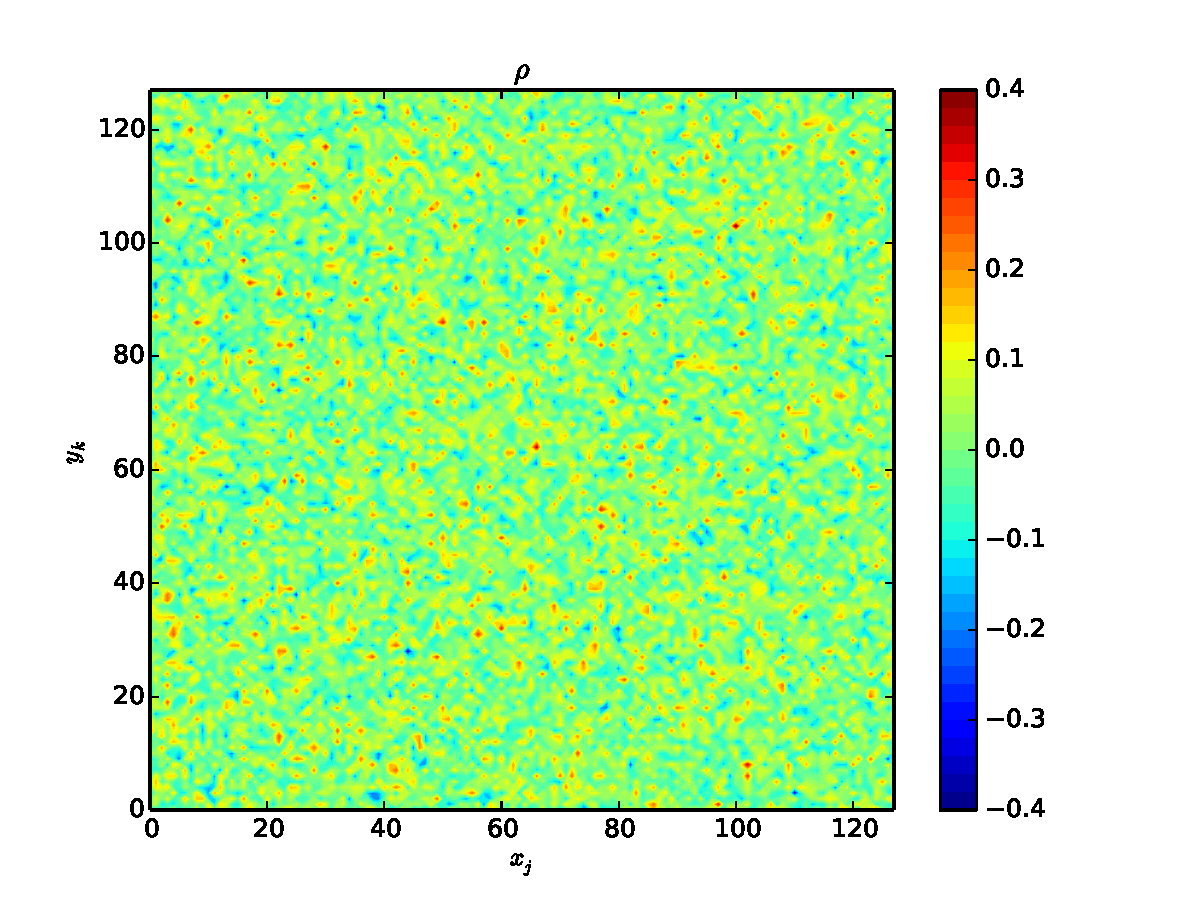
\includegraphics[width = \textwidth]{figures/verification/analytical/random/rho.pdf}
			\end{subfigure}
			\begin{subfigure}[b]{0.6\textwidth}
				\includegraphics[width = \textwidth]{figures/verification/analytical/random/numerical.pdf}
			\end{subfigure}
			\begin{subfigure}[b]{0.6\textwidth}
				\includegraphics[width = \textwidth]{figures/verification/analytical/random/residual.pdf}
			\end{subfigure}
			\caption{As earlier this is a \(x,y\)-plane cut along \(x_k=32\), of the grid. The plots show the charge distribution,
			numerical solution and the solution, from top to bottom. It is visible that the potential shows more structure than
			the \(\rho\), since the integration smooths the original problem.}
			\label{fig:random}
		\end{figure}

	\subsection{Additional Tests}
		In addition to the tests on shown in this section, we also ran the same tests
		obtaining similar results on various sizes and directions. Since we wanted to be sure that the program
		was working independently of the how the domain was divided into subdomains, we also performed
		tests on different subdomain divisions.


	\subsection{ND vs 3D algorithms}
		PINC is built to have two sets of algorithms, one N-dimensional and one 3-dimensional.
		The N-dimensional algorithms is meant to be used in cases where one want to do 1- and 2-dimensional
		simulations as well as a test for the 3-dimensional algorithm. The 3-dimensional algorithm
		is generally slightly faster than the N-dimensional due to some extra capabilities in hardcoding
		certain parts. On a laptop, using two 'Intel(R) Core(TM) i7-4710MQ CPU @ 2.50GHz' processors, we
		ran the multigrid solver on a \(128,128,128\) size problem, with both the \(3\)D and ND algorithms.
 		The ND algorithms used \(80.08\)s to solve it to the given tolerance, while the \(3\)D algorithms
 		used \(78.75\)s achieving only a slight speedup. This is likely due to most of the
		computational time being spent on the interprocessor communication.

    \section{Scaling of the error compared to discretization}
The solver is solving a discretized problem, due to this the solution will not
be exact. The error will be of second order, \(\order{h^2}\), dependent on the
stepssize, \(h\), due to the first order solver, see \cref{sec:GSRB}.


To investigate that the error the of the solver follows a second order improvement
as the stepsize decreases we construct a sinusoidal rho as a test case.

\begin{equation}
    \rho(x) = \sin{\left(\frac{x}{2\pi}\right)}      \qquad ; \qquad x\epsilon[0,2\pi]
\end{equation}

This \(\rho\) is analytically solvable for the Poisson equation so we can compute the
\(2\)-norm of the error, \(\norm{err}_2\). Then we gradually decrease the stepsize
and obtain and compare the norm of the numerical solutions. Since the normalization in PinC
is normally done outside the multigrid solver, \(rho\) had to be suitably scaled
to the stepsize. We expect the error proportional to \(h^2\), so by taking the logarithm
we obtain

\begin{equation}
    \log(err(h)) = 2\log(Ch)
\end{equation}

where \(C\) is a constant dependent on \(\rho\).

\begin{figure}
    \centering
    \begin{subfigure}[b]{0.49\textwidth}
        \includegraphics[width = \textwidth]{figures/verification/errorScaling/errorloglog}

    \end{subfigure}
    \begin{subfigure}[b]{0.49\textwidth}
        \includegraphics[width = \textwidth]{figures/verification/errorScaling/errorEloglog}
    \end{subfigure}
    \caption{Logarithmic plot of the 2-norm of the error of the potential \(\phi\), left figure, and the
    x-component of the electric field. The solver was run on a scaled sinus-shaped charge distribution.
    Both of the plots show a straight line of the error, on the logarithmic plots, with a slope
    of \(2.00\). This correspond to maximal error of \(\order{h^2}\)}
\end{figure}

    \subsection{Langmuir Oscillation Test Case}
As a test of the validity of our PiC program, we can use the langmuir wave
oscillation. This test is inspired by a case set up in \citet{birdsall_plasma_2004},
and modified to fit with our normalization and discretizations.

    \section{Plasma Oscillation}
\begin{itemize}
    \item Plasma oscillates
    \item Randomly distributed plasma, with random velocities (Vel Causing a bug->Fix)
    \item Compute fitting Temperature and Debye length
\end{itemize}

    \subsection{Input parameters}
        \subsubsection{Timestep}
        First we need to ensure that the simulation is does not violate the time-
        stability criterion, \cref{sec:time_stability}, \(\Delta t \leq 2\omega_{pe}\).
        For computational reasons each particle in the program represents many real particles
        and we can adjust the number, of real particles represented, to ensure
        that the electron plasma frequency is \(1\).

        \begin{equation}
            \omega_{pe}^2 = \frac{nq^2_e}{m\epsilon_0} = \left(\frac{N}{V}\right)\left(\frac{q_{e*}}{m_{e*} }\right)q_{e*}
        \end{equation}

        Here \((N/V)\) is just the number of electron super-particles divided by the volume,
        \(q_e\) and \(m_e\), represents super-particles and needs to be multiplied by the number
        of particles in a super-particle, \(\kappa\).

        \begin{equation}
            \omega_{pe}^2 = \left(\frac{N}{V}\right)\left(\frac{e}{m_e}\right)\kappa e
        \end{equation}

        Since we want the electron plasma frequency to be \(1\), \(\kappa\) is set to

        \begin{equation}
            \kappa = \frac{Vm_e}{Ne^2}
        \end{equation}

        Now the time is given in units of \(\omega_{pe}\) and we use \(\Delta t = 0.2 < 2\) easily.

        \subsubsection{Spatial-step}
        The spatial step need to satisfy the finite grid instability condition,
        \(\Delta x < \varsigma \lambda_{Se}\), \cref{sec:finite_grid_instability}.
        We use a similar procedure as in normalizing the time with regards to \(\omega_{pe}\)
        to normalize the length with regards to \(\lambda_{Se}\). The we end up with
        the temperature, or its other representation as thermal velocity, as the parameter we can adjust to make sure that it satisfies the
        condition.

        \begin{equation}
            \lambda_{Se}^2 = \frac{\epsilon_0 kT_e}{nq^2_e}
        \end{equation}

	\section{Performance}
    \section{Scaling}
  In this section we investigate the performance of the solver and different scaling
  measurements. We are interested in both how well the solver performs on a larger
  number of processors, as well as the perfomance impact of the different
  parameters in the solver.

  We want to obtain a better understanding of how the field resolution can be scaled
  up without hampering the perfomance of the particle-in-cell simulation to much.

  

    \subsection{Convergence Rate}
	As an iterative solver a multigrid solver will gradually approach a solution,
	reducing the residual further each run. In this subsection we will measure the convergence
	rate, defined in similar way as in \citet{zhukov_parallel_2014},
	%
	\begin{equation}
		p = \left(\frac{r_m}{r_0}\right)^{1/m}
	\end{equation}
	%
	where \(r_m, r_0\) are the \(2\)-norm of a the residual after \(m\) multigrid runs
 	and the inital residual. We presume that each run of the multigrid solver will
	remove a proportion of the remaining residual.
	The tests are done on a \(128^3\) grid on a sinusoidal
	problem, and the smoothers run for an equal number of runs on each level.
	%
	(Table of convergence rate numbers)
	%
	\citeauthor{zhukov_parallel_2014} found convergence rates of \(p \approx 0.15\) and \(p \approx 0.17\)
	using a multigrid solver with a Chebyshev algorithm to smooth.

    \subsection{Scaling of the MG Solver}
	One of the aims of building a parallell multigrid solver was to be able
	to enable simulating large plasma problems. To be able to achieve that the solver
	should be able to scale up very well, i.e. doubling the problem size and the number
	of available processors should only give a manageable increase in computational time.
	We don't expect to be able to achieve a perfect parallelization, since there is
	a certain amount of interprocessor communications necessary that will slow down
	the algorithm compared to a sequential algorithm. The exact parallel performance
	is also dependent on the communications channels and the topology between the processor clusters.
	In \cref{sec:para_comp} the parallel
	complexeties for the different multigrd algorithms is given and we will look at
	the parallel proprties for a V, W and FMG algorithm.


	To investigate the scaling properties we will run set up a standard problem,
	and solve it with increasing resolutions. We keep the size of the domain unchanged but increase the resolution (reducing the spacing). We start with a \(32^3\) grid on
 	\(1^3\) computaional core, then we increase the problemsize to \(64^3\) on \(2^3\)
	and so on. These tests were run on Abel, UiO's computer cluster, and the technical details
	can be found at the web page \footnote{http://www.uio.no/english/services/it/research/hpc/abel/more/index.html (Accessed 2016-11-15)}.
	The results are shown on c\ref{fig:scalingMG}.
	%
	\begin{figure}
		% \begin{subfigure{\textwith}
		\label{fig:scalingMG}
		\includegraphics[width = \textwidth]{figures/performance/scalingMG}
		\caption{A Langmuir Oscillation were performed for \(10\) timesteps with a \((32,32,32)\) grid on each processor.
		This was repeated with increasing amount of processors, \((1, 8, 32, 64)\), to see how the multigrid solver scales.}
		% \end{subfigure}
	\end{figure}
	%
	%Comments
	From \cref{sec:para_comp} we expect theoretical optimal scaling of \(\log{N}\log{\varepsilon}\).
	While this was not achieved, the settings were not optimized in these runs, for the various problem sizes and
	this may have caused it to scale worse than it should. When more processors are used the speed of
	the interprocessor communcation may have slowed down, as the processors are not part of the
	same node. The main problem with the test was that the subdomains was very small so
	the communication costs dominated. The communication costs scales linearly \citep{jung_parallelization_1997}, so
	for the coarse grids of the \(5\)-level multigrid the solver scaled close to linearly.

	\citet{baker_scaling_2012} found it crucial to use assumed partition
	to achieve good scalability, as the interprocessor communication costs are the main obstacle to
	scalability for multigrid methods. By assumed partitioning the subdomains are divided into nearby groups
	to easy communication between them.

    % \subsection{Scaling Multigrid vs PINC}
	As well as the scaling properties of the multigrid solver a look at the
	whole PiC model is interesting. This helps us easier pinpoint where further
	optimizations efforts should be directed. We do not necessarilly except the
	the particle based algorithms to scale up to larger problems in the same
	rate as	the solver. So above a certain number of processors, or size, there may
	be a bottleneck.

	\begin{table}
		\begin{tabular}{c | c | c}
		&	Multigrid & Total\\
		\\ \hline 
		\end{tabular}
	\end{table}


\chapter{Summary and Conclusion}
	\label{sec:summ}
	
\section{Summary}
	The main object of this project was to develop a new parallel multigrid solver
	for use in PINC.

	The verification section goes through the different ways the
	solver was tested. The main tests were done on charge distributions
	with known analytical solutions. The numerical solutions where confirmed to
 	agree with the analytical solutions. These type of tests where done for various
	dimensions and subdivisions of the domain. The \(N\)-dimensional algorithms were
	then tested and compared with the specialized \(3\)-dimensional algorithms. For the chosen
	parameters the \(N\)-dimensional algorithms were almost as fast as the \(3\)D version, this may not be true
	for all configurations. Unfortunately the capability of the solver to use different boundary conditions, and mix them,
 	was not well tested due to bad time management.
	The \(\order{h^2}\) scaling of the \(1\)st order discretization of the solver
 	was then verified by measuring how the error decreased as the resolution increased.
	Next we wanted to look at the whole PINC program. It then confirmed to work correctly
	with a simulation of a Langmuir Oscillation.

	Since PINC is made to performon a supercomputer we wanted to see how well it
	performs and scales on a multiple processors. First we measured the convergence rate of the algorithm,
	which was found to be For this we used UiO's supercomputer Abel.
	Due to bad choices in multigrid parameters, using \(5\) multigrid levels on small grids, the communication
	dominated the computational time. Due to time constraints further scaling measurements with better
	parameters were not conducted.



\section{Concluding Remarks and Further Proposals}
	While the multigrid solver was shown to work and produce the correct results the scalability
	was satisfactorily shown. While the program is usable and under further development, it needs to be shown
	to scale well. A multigrid algorithm based on Gauss-Seidel should scale better than the performed tests show,
	as \citet{jung_parallelization_1997} showed. It should also be considered to implement the \textit{processor-block Gauss-Seidel}
	from \citet{adams_parallel_2003}. Further additions to increase the possible use of PINC include
	the possiblity to have objects in the plasma, which can be used to model the effects surrounding space craft
	and dust particles \citep{miloch_wake_2010,miyake_plasma_2013,ergun_spacecraft_2010}. Collisions
	between particles will enable further studies of instabilities of plasma streams \citep{brackbill_particle_1995}.
	Another way PINC can be further developed is with full implicit algorithms.  



%
\appendix
% \chapter{Further Development}
%     Here is a list of what possible improvements and extensions that we hope
is eventually developed in our PinC program. Our aim was to develop a solid, basic
and easy to use parallel PiC program, that is suited to further development. Our hope
is that this project eventually develops into a full scale open source PiC program.

\begin{itemize}
    \item Objects
    \item Adaptive mesh
    \item Realtime plasma vizualizations (ala Atomify)
    \item Full Electromagnetic PiC
    \item Compatibility with FEM (dolphin) as a solver
    \item Hybrid, add on possibility of fluid-species and molecular dynamics
    \item Spectral Solvers (Wish that was available for testing of other solvers)
    \item Variable Ghost Layers
    \item Various stencils, interpolation and discretizations of different orders
\end{itemize}

%
% \chapter{Notation}
%     \section{Notation}
  While the notation is described in the main text at its first instance, we have also included
  this small note on the notation used to make it easier to look up.
  Notation that are only used in locally in smaller sections are not included here.

  In the PinC project we have decided to try to keep different indexes tied different
  objects to help avoid confusion and increase readability. Since the \(i\) index is
  reserved for incrementing particles, the spatial \(x,y,z\)-indexes are \(j,k,l\) instead of the
  more usual \(i,j,k\). So to make the transition between this document and the code
  easier we have also used the \(j,k,l\) indexes to denote the spatial area.
  This is the convention used by Birdsall and Langdon, (cite plasma physics via simulation).


  Subscripts are usually used to denote spatial index, and a superscripts are usually
  reserved for temporal cases. So \( \Phi^n_{j,k,l} \) means the potential at
  the timestep \(n\) and position \(j,k,l\). When plasma theory is involved the subscript
  can also signify the particle species.


  \begin{centering}
    \begin{tabular}{c |l}
      \(\Phi\) & Electric Potential
      \\
      \(\rho\) & Charge Density
      \\
      \omega_{pe} & Electron Plasma Frequency
      \\
      \omega_{ce} & Electron Cycletron Frequency
      \\
      T_e   & Electron Kinetic Temperature
      \\
      \vb{E}    & Electric Field
      \\
      \vb{B}    & Magnetic Field
      \\
      \vb{r}    & Position
      \\
      m         & Mass
      \\
      T         & Kinetic Temperature
    \end{tabular}
  \end{centering}

%
\chapter{Unittests}
    \section{Unittests}
\label{sec:unittests}
Unittests are small tests that is used to check that the single pieces of the code
work as they should. This serves a dual purpose in developing a software project.
When a part of the code is developed it serves as a framework to create a standardized
test of the piece of code that can easily be repeated. The unit tests are not maintained
in the latest version of the software.
It also helps when developing the higher level algorithms, in that the unittests ensures
that the problem lies in the higher level algorithm and not in the lower level pieces
it uses. When implementing wider changes, for example datastructures, the unittests
can help making sure that the changes are not causing any unintended bugs. For
information of how to use the unittests see the documentation, \cite{documentation}.

\subsection{Prolongation and Restriction}
	The prolongation and restriction operators with the earlier proposed stencils
  will average out the grid points when applied. So the idea here is to set up a
  system with a constant charge density, \(\rho(\va{r}) = C\), and then apply a
  restriction. After performing the restriction we can check that the grid points
  values are preserved. Then we can do the same with the prolongation. While this
  does not completely verify that the operators work as wanted, it gives an indication
	that we have not lost any grid points and the total mass of the charge density should be conserved.

\subsection{Finite difference}
  The finite difference operators is tested by setting up a test
  field based on a polynomial on which the operator should give an exact answer for.
  For example if we have a quantity \(f(x) = 3x\), then a first order finite difference
  scheme will give \(\hat{\nabla}f(x) = 3\).

\subsection{Multigrid and Grid structure}
  We want the basic grid to be available through a grid datastructure and the stack
  of grids stored in the multigrid structure. To ensure that this will still work
  through changes in the the structs there is a simple unittest that uses a grid struct
  to set up a field, then it is changed in the multigrid struct. Then it confirms
  that the values in the grid struct is also changed.

\subsection{Edge Operations}
  In the communication between the subdomains, as well as in the treatment of
  boundary conditions, there is a group of functions dealing with slice operations.
  These are tested by putting assigning each subdomain different constant values,
  then different slice operations is performed.

\chapter{Scripts}
	\section{PINC framework}
\begin{lstlisting}[language=python, caption = Framework to more easily run PINC with various settings]

import subprocess
import numpy as np

class Pinc(dict):
	def __init__(self, pinc="./mpinc.sh", ini="langmuirWarm.ini", path="../.."):
		# All commands will be executed from "path"

		self.pinc = pinc
		self.ini = ini
		self.path = path

	def run(self):
		cmd = self.pinc + " " + self.ini
		for key in self:
			cmd += " " + key + "=" + self.parse(key)
		self.runCommand(cmd)

	def runCommand(self, cmd):
		cmd = "cd " + self.path + "; " + cmd
		subprocess.call(cmd,shell=True)

	def clean(self):
		self.runCommand("rm -f data/*.h5")
		self.runCommand("rm -f data/*.txt")

	def parse(self, key):
		value = self[key]
		if isinstance(value,(list,np.ndarray)):
			string = str(value[0])
			if(len(value) > 1):
				for l in range(1,len(value)):
					string += "," + str(value[l])
			return string
		elif isinstance(value,(int,float)):
			return str(value)
		else:
			return value
		\end{lstlisting}


\section{Multigrid Parameter Optimizer}
\label{sec:optimizer}
\begin{lstlisting}[language=python, caption = Optimizer script]
	from pincClass import *
import subprocess
import h5py
import numpy as np
import sys as sys

if(len(sys.argv) > 1):
	path = "../../" + sys.argv[1]
else:
	path = "../../local.ini"
pinc = PINC(iniPath = path)

#Setting up wanted needed ini file
pinc.mode 		= "mgRun"
pinc.mgCycles 		= 1
pinc.startTime		= -1

class Settings:
	def __init__(self, nPre = 10, nPost = 10,
					nCoarse = 10, mgLevels = 3):
		self.nPre    	= nPre
		self.nPost   	= nPost
		self.nCoarse 	= nCoarse
		self.mgLevels	= mgLevels
		#Store results
		self.mgCycles 	= 0
		self.time 		= float('Inf')

	def copy(self, copy):
		self.nPre 		= copy.nPre
		self.nPost		= copy.nPost
		self.nCoarse	= copy.nCoarse
		self.mgLevels 	= copy.mgLevels

	def setPinc(self, pinc):
		pinc.preCycles 			= self.nPre
		pinc.postCycles			= self.nPost
		pinc.coarseCycles		= self.nCoarse
		pinc.mgLevels 			= self.mgLevels
		pinc.startTime 			+= 1


def formatTimeCycles(fileName, nRuns):
	data = h5py.File(fileName,'r')
	time = np.array(data['time'][nRuns,1])
	mgCycles= np.array(data['cycles'][nRuns,1])
	data.close()

	return time, mgCycles


def nCycleOptimize(count, nTries, nRun, bestRun, currentRun, pinc):
	pTime = float('Inf')
	preInc = 1
	for j in range(0,nTries): #nCoarse
		# print "Hello"
		if(count>0):
			nRun = nCycleOptimize(count -1, nTries, nRun, bestRun, currentRun, pinc)
		##Run, retrieve time and cycles used
		currentRun.setPinc(pinc)
		pinc.runMG()
		time, mgCycles = formatTimeCycles('test_timer.xy.h5',nRun)

		#Check if best run
		if(time < bestRun.time):
			bestRun.copy(currentRun)
			bestRun.time = time
			bestRun.mgCycles = mgCycles

		if(preInc == 1):
			if(time < pTime):
				pTime = time
				if(count == 2):
					currentRun.nCoarse *= 2
				if(count == 1):
					currentRun.nPre *= 2
				if(count == 0):
					currentRun.nPost *=2
			else:
				if(count == 2):
					currentRun.nCoarse *= 0.5
				if(count == 1):
					currentRun.nPre *= 0.5
				if(count == 0):
					currentRun.nPost *=0.5
				preInc = -1
		else:
			if(time < pTime):
				pTime = time
				if(count == 2):
					currentRun.nCoarse *= 0.5
				if(count == 1):
					currentRun.nPre *= 0.5
				if(count == 0):
					currentRun.nPost *=0.5
			else:
				break
		nRun += 1
	return nRun


bestRun = Settings()
currentRun = Settings(10,10,10,5)

pinc.clean()
nTries 	= 100
nRun	= 0
preInc 	= 1



for i in range(1):	#mgLevels

	# nRun = nCoarseOpt(nTries, nRun, bestRun, currentRun, pinc)
	nRun = nCycleOptimize(2 ,nTries, nRun, bestRun, currentRun, pinc)

	currentRun.mgLevels += 1


print "\nBest runtime \t= "	, bestRun.time*1.e-9, "s"
print "\nProposed run:"
print "mgCycles \t= "		, bestRun.mgCycles
print "mgLevels \t= "		, bestRun.mgLevels
print "nPreSmooth \t= "		, bestRun.nPre
print "nPostSmooth \t= "	, bestRun.nPost
print "nCoarseSolve \t= "	, bestRun.nCoarse

\end{lstlisting}

\subsection{V-cycle, code}
\label{sec:mg_V}
\begin{lstlisting}[language=c, caption = Implementation of an recursive V-cycle]
void inline static mgVRecursive(int level, int bottom, int top, Multigrid *mgRho, Multigrid *mgPhi,
								Multigrid *mgRes, const MpiInfo *mpiInfo){

//Solve and return at coarsest level
if(level == bottom){
	gInteractHalo(setSlice, mgPhi->grids[level], mpiInfo);
	mgRho->coarseSolv(mgPhi->grids[level], mgRho->grids[level], mgRho->nCoarseSolve, mpiInfo);
	mgRho->prolongator(mgRes->grids[level-1], mgPhi->grids[level], mpiInfo);
	return;
}

//Gathering info
int nPreSmooth = mgRho->nPreSmooth;
int nPostSmooth= mgRho->nPostSmooth;

Grid *phi = mgPhi->grids[level];
Grid *rho = mgRho->grids[level];
Grid *res = mgRes->grids[level];

//Boundary
gInteractHalo(setSlice, rho, mpiInfo);
gBnd(rho,mpiInfo);

//Prepare to go down
mgRho->preSmooth(phi, rho, nPreSmooth, mpiInfo);
mgResidual(res, rho, phi, mpiInfo);
gInteractHalo(setSlice, res, mpiInfo);
gBnd(res, mpiInfo);

//Go down
mgRho->restrictor(res, mgRho->grids[level + 1]);
mgVRecursive(level + 1, bottom, top, mgRho, mgPhi, mgRes, mpiInfo);

//Prepare to go up
gAddTo( phi, res );
gInteractHalo(setSlice, phi,mpiInfo);
gBnd(phi,mpiInfo);
mgRho->postSmooth(phi, rho, nPostSmooth, mpiInfo);

//Go up
if(level > top){
	mgRho->prolongator(mgRes->grids[level-1], phi, mpiInfo);
}
return;
}
\end{lstlisting}

%
\chapter{Examples}
    \section{Ex: 3 level V cycle, steps necessary}
	\label{sec:EX_V_Ccyles}
\begin{dingautolist}{192}
			\item Compute defect on grid \(0\), the finest grid:
		\begin{itemize}
			\item	\( \widehat{\phi}_0 = \mathcal{S}(\phi_0, \rho_0)\)
			\item 	\(d_0 = \nabla^2\widehat{\phi}_0 - \rho_0\)
			\item Restrict defect: \(\rho_1 = \mathcal{R}d_0 \) \nonumber
		\end{itemize}
	\item Compute defect on grid \(1\):
		\begin{itemize}
			\item \(\widehat{\phi}_1 = \mathcal{S}(\phi_1^0, \rho_1)\)
			\item \(d_1 = \nabla^2\widehat{\phi}_1 - \rho_1 \)
			\item Restrict defect: \(\rho_2 = \mathcal{R}d_1 \)
		\end{itemize}
	\item Solve Coarse Grid for correction \(\omega\)
		\begin{itemize}
			\item \( \phi_2 = \mathcal{S}(\phi_2^0, \rho_2)\)
			\item Interpolate as correction:\(\omega_1 = \mathcal{I}\phi_2\)
		\end{itemize}
	\item Add correction on level 1:
		\begin{itemize}
			\item \(\widetilde{\phi}_1 = \widehat{\phi}_1 + \omega_1\)
			\item \( \phi_1 = \mathcal{S}(\widetilde{\phi}_1, \rho_1)  \)
			\item Interpolate correction:\( \omega_0 = \mathcal{I} \phi_1\)
		\end{itemize}
	\item Compute solution.
		\begin{itemize}
			\item \(\widetilde{\phi}_0 = \widehat{\phi}_0 + \omega_0\)
			\item \( \phi_0 = \mathcal{S}(\widetilde{\phi}_0, \rho_0)  \)
		\end{itemize}
\end{dingautolist}

% \chapter{Optional methods}
%     \input{chapters/appendix/alt_methods}
\chapter{Multigrid Libraries}
    

Efficient computation of the poisson equation, or other elliptic equations, is a common problem with many applications, and there exists several predeveloped and optimized libraries to help solve it. These include Parallel Particle Mesh (PPM) \citep{sbalzarini_ppm_2006}, Hypre \citep{falgout_hypre:_2002}, Muelu (), METIS \citep{_fast_????} and PETCs \citep{_manual.pdf_????} amongst others. There is also PiC libraries that can be used PICARD and VORPAL to mention two.

If we want to have an efficient integration of a multigrid library into our PiC model we need to consider how easy it is to use with our scalar and field structures. To have an effiecient program we need to avoid having the program convert data between our structures and the library structures. Since our PiC implementation uses the same datastructures for the scalar fields in several other parts, than the solution to the poisson equation, we could have an efficiency problem in the interface between our program and the library.

We could also consider that only part of the multigrid algorithm uses building blocks from libraries. The algorithm is now using the conceptually, and programatically easy, GS-RB as smoothers, but if we implement compatibility with a library we could easily use several other types of smoothers which could improve the convergence of the algorithm

\section{Libraries}

\section{PPM - Parallel Particle Mesh}
Parallel Particle Mesh is a library designed for particle based approaches to physical problems, written in Fortran. As a part of the library it includes a structured geometric multigrid solver which follows a similar algorithm to the algorithm we have implemented in our project implemented in both 2 and 3 dimensions. For the 3 dimensional case the laplacian is discretized with a \(7\)-point stencil, then it uses a RB-SOR (Red and Black Succesive Over-Relaxation), which equals GS-RB with the relaxation parameter \(\omega\) set as \(1\), as a smoother. The full-weighting scheme is used for restriction and trilinear interpolation for the prolongation, both are described in \citep{trottenberg_multigrid_2000}. It has implementations for both V and W multigrid cycles. To divide up the domains between the computational nodes it uses the METIS library. The efficiency of the parallel multigrid implementation was tested

\section{Hypre}
Hypre is a library developed for solving sparse linear systems on massive parallel computers. It has support for c and Fortran. Amongst the algorithms included is both structured multigrid as well as element-based algebraic multigrid. The multigrid algorithms scales well on up to \(100 000\) cores, for a detailed overview see Baker et. al. (2012).

\section{MueLo - Algebraic Multigrid Solver}
MueLo is an algebraic multigrid solver, and is a part of the TRILINOS project and has the advantage that it works in conjunction with the other libraries there. It is written as an object oriented solver in cpp. For a investigation into the scaling properties see Lin et. al. (2014).


\section{METIS - Graph Partitioning Library}
METIS is a library that is used for graph partitioning, and could have been used in our program to partition the grids. The partitionings it produces has been shown to be \(10\%\) to \(50\%\) faster than the partionionings produces by spectral partitioning algorithms \citep{_fast_????}. It is mostly used for irregular graphs, and we are not sure if it could be easily made to work with the datastructures used throughout the program.


\section{PETSc - Scientific Toolkit}
The PETSc is an extensive toolkit for scientific calculation that is used by a multitude of different numerical applications, including FEniCS. It has a native multigrid option, DMDA, where the grid can be constructed as a cartesian grid. In addition there is large amount of inbuilt smoothers that can be used.


% \chapter{Code}
%     %%%%%%%%%%%%%%%%%%%%%%%%%MG-Cycles%%%%%%%%%%%%%%%%%%%%%%%%%%%%%%%%%%%%%%%%%%%
\newpage
	\subsection{V-cycle, code}
	\label{sec:mg_V}
	\begin{lstlisting}[language=c, caption = Implementation of an recursive V-cycle]
void inline static mgVRecursive(int level, int bottom, int top, Multigrid *mgRho, Multigrid *mgPhi,
 									Multigrid *mgRes, const MpiInfo *mpiInfo){

	//Solve and return at coarsest level
	if(level == bottom){
		gInteractHalo(setSlice, mgPhi->grids[level], mpiInfo);
		mgRho->coarseSolv(mgPhi->grids[level], mgRho->grids[level], mgRho->nCoarseSolve, mpiInfo);
		mgRho->prolongator(mgRes->grids[level-1], mgPhi->grids[level], mpiInfo);
		return;
	}

	//Gathering info
	int nPreSmooth = mgRho->nPreSmooth;
	int nPostSmooth= mgRho->nPostSmooth;

	Grid *phi = mgPhi->grids[level];
	Grid *rho = mgRho->grids[level];
	Grid *res = mgRes->grids[level];

	//Boundary
	gInteractHalo(setSlice, rho, mpiInfo);
	gBnd(rho,mpiInfo);

	//Prepare to go down
	mgRho->preSmooth(phi, rho, nPreSmooth, mpiInfo);
	mgResidual(res, rho, phi, mpiInfo);
	gInteractHalo(setSlice, res, mpiInfo);
	gBnd(res, mpiInfo);

	//Go down
	mgRho->restrictor(res, mgRho->grids[level + 1]);
	mgVRecursive(level + 1, bottom, top, mgRho, mgPhi, mgRes, mpiInfo);

	//Prepare to go up
	gAddTo( phi, res );
	gInteractHalo(setSlice, phi,mpiInfo);
	gBnd(phi,mpiInfo);
	mgRho->postSmooth(phi, rho, nPostSmooth, mpiInfo);

	//Go up
	if(level > top){
		mgRho->prolongator(mgRes->grids[level-1], phi, mpiInfo);
	}
	return;
}
	\end{lstlisting}

\newpage
\begin{lstlisting}[language=c, caption = Implementation of an recursive V-cycle]
void mgVRegular(int level, int bottom, int top, Multigrid *mgRho, Multigrid *mgPhi,
 									Multigrid *mgRes, const MpiInfo *mpiInfo){

	//Gathering info
	int nPreSmooth = mgRho->nPreSmooth;
	int nPostSmooth= mgRho->nPostSmooth;
	int nCoarseSolv= mgRho->nCoarseSolve;


	//Down to coarsest level
	for(int current = level; current <bottom; current ++){
		//Load grids
		Grid *phi = mgPhi->grids[current];
		Grid *rho = mgRho->grids[current];
		Grid *res = mgRes->grids[current];

		//Boundary
		gInteractHalo(setSlice, phi,mpiInfo);
		gBnd(phi,mpiInfo);

		mgRho->preSmooth(phi, rho, nPreSmooth, mpiInfo);
		mgResidual(res, rho, phi, mpiInfo);
		mgRho->restrictor(res, mgRho->grids[current + 1]);
	}

	//Solve at coarsest
	gInteractHalo(setSlice, mgRho->grids[bottom], mpiInfo);
	gBnd(mgRho->grids[bottom],mpiInfo);
	mgRho->coarseSolv(mgPhi->grids[bottom], mgRho->grids[bottom], nCoarseSolv, mpiInfo);
	mgRho->prolongator(mgRes->grids[bottom-1], mgPhi->grids[bottom], mpiInfo);

	//Up to finest
	for(int current = bottom-1; current >-1; current --){
		//Load grids
		Grid *phi = mgPhi->grids[current];
		Grid *rho = mgRho->grids[current];
		Grid *res = mgRes->grids[current];


		//Prepare to go up
		gAddTo( phi, res );
		gInteractHalo(setSlice, phi,mpiInfo);
		gBnd(phi,mpiInfo);
		mgRho->postSmooth(phi, rho, nPostSmooth, mpiInfo);
		if(level > top)	mgRho->prolongator(mgRes->grids[current-1], phi, mpiInfo);
	}

	return;
}
\end{lstlisting}


%%%%%%%%%%%%%%%%%%%%%%%%%Prolongators/Restrictors%%%%%%%%%%%%%%%%%%%%%%%%%%%%



%%%%%%%%%%%%%%%%%%%%%%%%%Iterative Solvers%%%%%%%%%%%%%%%%%%%%%%%%%%%%%%%%%%%
\newpage
\section{Iterative solvers}
\subsection{Jacobian code}
\label{sec:jacobian}

\begin{lstlisting}[language=c, caption = Code snippet 2D jacobian]
  for(int c = 0; c < nCycles; c++){
    // Index of neighboring nodes
    int gj = sizeProd[1];
    int gjj= -sizeProd[1];
    int gk = sizeProd[2];
    int gkk= -sizeProd[2];

    for(long int g = 0; g < sizeProd[rank]; g++){
      tempVal[g] = 0.25*(	phiVal[gj] + phiVal[gjj] +
                phiVal[gk] + phiVal[gkk] + rhoVal[g]);

      gj++;
      gjj++;
      gk++;
      gkk++;
    }

    for(int q = 0; q < sizeProd[rank]; q++) phiVal[q] = tempVal[q];
    for(int d = 1; d < rank; d++) gSwapHalo(phi, mpiInfo, d);
  }
\end{lstlisting}

\newpage
\subsection{GS-RB 2D}
\label{sec:GS_RB_2D}
\begin{lstlisting}[language=c, caption = Main loop]
    for(int c = 0; c < nCycles;c++){

      //Increments
      int kEdgeInc = nGhostLayers[2] + nGhostLayers[rank + 2] + sizeProd[2];

      /**************************
       *	Red Pass
       *************************/
      //Odd numbered rows
      g = nGhostLayers[1] + sizeProd[2];
      loopRedBlack2D(rhoVal, phiVal, sizeProd, trueSize, kEdgeInc, g, gj, gjj, gk, gkk);

      //Even numbered columns
      g = nGhostLayers[1] + 1 + 2*sizeProd[2];
      loopRedBlack2D(rhoVal, phiVal, sizeProd, trueSize, kEdgeInc, g, gj, gjj, gk, gkk);

      for(int d = 1; d < rank; d++) gSwapHalo(phi, mpiInfo, d);

      /***********************************
       *	Black pass
       **********************************/
      //Odd numbered rows
      g = nGhostLayers[1] + 1 + sizeProd[2];
      loopRedBlack2D(rhoVal, phiVal, sizeProd, trueSize, kEdgeInc, g, gj, gjj, gk, gkk);

      //Even numbered columns
      g = nGhostLayers[1] + 2*sizeProd[2];
      loopRedBlack2D(rhoVal, phiVal, sizeProd, trueSize, kEdgeInc, g, gj, gjj, gk, gkk);


      for(int d = 1; d < rank; d++) gSwapHalo(phi, mpiInfo, d);
    }

    return;
  }
\end{lstlisting}

\begin{lstlisting}[language=c, caption = Loop through grid]
  gj = g + sizeProd[1];
  gjj= g - sizeProd[1];
  gk = g + sizeProd[2];
  gkk= g - sizeProd[2];

  for(int k = 1; k < trueSize[2]; k +=2){
    for(int j = 1; j < trueSize[1]; j += 2){
      phiVal[g] = 0.25*(	phiVal[gj] + phiVal[gjj] +
                phiVal[gk] + phiVal[gkk] + rhoVal[g]);
      g	+=2;
      gj	+=2;
      gjj	+=2;
      gk	+=2;
      gkk	+=2;
    }
    g	+=kEdgeInc;
    gj	+=kEdgeInc;
    gjj	+=kEdgeInc;
    gk	+=kEdgeInc;
    gkk	+=kEdgeInc;
  }
\end{lstlisting}

\newpage
\subsection{GS-RB 3D if tests}
\label{sec:GS-RB_if}
\begin{lstlisting}[language=c, caption = GS-RB with if-tests]

  /*********************
   *	Red Pass
   ********************/
  g = sizeProd[3]*nGhostLayers[3];
  for(int l = 0; l < trueSize[3];l++){
    for(int k = 0; k < size[2]; k++){
      for(int j = 0; j < size[1]; j+=2){
        phiVal[g] = 0.125*(	phiVal[g+gj] + phiVal[g-gj] +
                  phiVal[g+gk] + phiVal[g-gk] +
                  phiVal[g+gl] + phiVal[g-gl] + rhoVal[g]);
        g	+=2;
      }
      if(l%2){
        if(k%2)	g+=1; else g-=1;
      } else {
        if(k%2) g-=1; else g+=1;
      }

    }
    if(l%2) g-=1; else g+=1;
  }

  for(int d = 1; d < rank; d++) gSwapHalo(phi, mpiInfo, d);
\end{lstlisting}

\newpage
\subsection{GS-RB 3D without if tests}
\begin{lstlisting}[language=c, caption = main routine]
/**************************
 *	Red Pass
 *************************/
//Odd layers - Odd Rows
g = nGhostLayers[1]*sizeProd[1] + nGhostLayers[2]*sizeProd[2] + nGhostLayers[3]*sizeProd[3];
loopRedBlack3D(rhoVal, phiVal, sizeProd, trueSize, kEdgeInc, lEdgeInc,
        g, gj, gjj, gk, gkk, gl, gll);

//Odd layers - Even Rows
g = (nGhostLayers[1]+1)*sizeProd[1] + (nGhostLayers[2]+1)*sizeProd[2] + nGhostLayers[3]*sizeProd[3];
loopRedBlack3D(rhoVal, phiVal, sizeProd, trueSize, kEdgeInc, lEdgeInc,
        g, gj, gjj, gk, gkk, gl, gll);

//Even layers - Odd Rows
g = (nGhostLayers[1])*sizeProd[1] + (nGhostLayers[2])*sizeProd[2] + (nGhostLayers[3]+1)*sizeProd[3];
loopRedBlack3D(rhoVal, phiVal, sizeProd, trueSize, kEdgeInc, lEdgeInc,
        g, gj, gjj, gk, gkk, gl, gll);

//Even layers - Even Rows
g = (nGhostLayers[1] + 1)*sizeProd[1] + (nGhostLayers[2]+1)*sizeProd[2] + (nGhostLayers[3]+1)*sizeProd[3];
loopRedBlack3D(rhoVal, phiVal, sizeProd, trueSize, kEdgeInc, lEdgeInc,
        g, gj, gjj, gk, gkk, gl, gll);

for(int d = 1; d < rank; d++) gSwapHalo(phi, mpiInfo, d);
\end{lstlisting}

\begin{lstlisting}[language=c, caption = loop routine]
  inline static void loopRedBlack3D(double *rhoVal,double *phiVal,long int *sizeProd, int *trueSize, int kEdgeInc, int lEdgeInc,
        long int g, long int gj, long int gjj, long int gk, long int gkk, long int gl, long int gll){

  gj = g + sizeProd[1];
  gjj= g - sizeProd[1];
  gk = g + sizeProd[2];
  gkk= g - sizeProd[2];
  gl = g + sizeProd[3];
  gll= g - sizeProd[3];

  for(int l = 0; l<trueSize[3]; l+=2){
    for(int k = 0; k < trueSize[2]; k+=2){
      for(int j = 0; j < trueSize[1]; j+=2){
        // msg(STATUS, "g=%d", g);
        phiVal[g] = 0.125*(phiVal[gj] + phiVal[gjj] +
                phiVal[gk] + phiVal[gkk] +
                phiVal[gl] + phiVal[gll] + rhoVal[g]);
        g	+=2;
        gj	+=2;
        gjj	+=2;
        gk	+=2;
        gkk	+=2;
        gl	+=2;
        gll	+=2;{subfigure}
      }
    g	+=kEdgeInc;
    gj	+=kEdgeInc;
    gjj	+=kEdgeInc;
    gk	+=kEdgeInc;
    gkk	+=kEdgeInc;
    gl	+=kEdgeInc;
    gll	+=kEdgeInc;
    }
  g	+=lEdgeInc;
  gj	+=lEdgeInc;
  gjj	+=lEdgeInc;
  gk	+=lEdgeInc;
  gkk	+=lEdgeInc;
  gl	+=lEdgeInc;
  gll	+=lEdgeInc;
  }

  return;
}
\end{lstlisting}



% \newpage
% NB! Note to self, page 122 has a proposed exact solution to u(x,y) = x+2y with no discretization errors. (In which document may I ask?)
% NB! Remember to cite mayavi if using their visualization package
%
\printbibliography

\end{document}
